
\NeedsTeXFormat{LaTeX2e}

\documentclass{jpp}

\usepackage{graphicx}
\usepackage{natbib}
\usepackage{epstopdf}

% See if the author has AMS Euler fonts installed: If they have, attempt
% to use the 'upmath' package to provide upright math.
\ifCUPmtlplainloaded \else
  \checkfont{eurm10}
  \iffontfound
    \IfFileExists{upmath.sty}
      {\typeout{^^JFound AMS Euler Roman fonts on the system,
                   using the 'upmath' package.^^J}%
       \usepackage{upmath}}
      {\typeout{^^JFound AMS Euler Roman fonts on the system, but you
                   dont seem to have the}%
       \typeout{'upmath' package installed. JPP.cls can take advantage
                 of these fonts, if you use 'upmath' package.^^J}%
       \providecommand\upi{\pi}%
      }
  \else
    \providecommand\upi{\pi}%
  \fi
\fi

% See if the author has AMS symbol fonts installed: If they have, attempt
% to use the 'amssymb' package to provide the AMS symbol characters.

\ifCUPmtlplainloaded \else
  \checkfont{msam10}
  \iffontfound
    \IfFileExists{amssymb.sty}
      {\typeout{^^JFound AMS Symbol fonts on the system, using the
                'amssymb' package.^^J}%
       \usepackage{amssymb}%
       \let\le=\leqslant  \let\leq=\leqslant
       \let\ge=\geqslant  \let\geq=\geqslant
      }{}
  \fi
\fi

% See if the author has the AMS 'amsbsy' package installed: If they have,
% use it to provide better bold math support (with \boldsymbol).

\ifCUPmtlplainloaded \else
  \IfFileExists{amsbsy.sty}
    {\typeout{^^JFound the 'amsbsy' package on the system, using it.^^J}%
     \usepackage{amsbsy}}
    {\providecommand\boldsymbol[1]{\mbox{\boldmath $##1$}}}
\fi

%%% Example macros (some are not used in this sample file) %%%

% For units of measure
\newcommand\dynpercm{\nobreak\mbox{$\;$dyn\,cm$^{-1}$}}
\newcommand\cmpermin{\nobreak\mbox{$\;$cm\,min$^{-1}$}}

% Various bold symbols
\providecommand\bnabla{\boldsymbol{\nabla}}
\providecommand\bcdot{\boldsymbol{\cdot}}
\newcommand\biS{\boldsymbol{S}}
\newcommand\etb{\boldsymbol{\eta}}

% For multiletter symbols
\newcommand\Real{\mbox{Re}} % cf plain TeX's \Re and Reynolds number
\newcommand\Imag{\mbox{Im}} % cf plain TeX's \Im
\newcommand\Rey{\mbox{\textit{Re}}}  % Reynolds number
\newcommand\Pran{\mbox{\textit{Pr}}} % Prandtl number, cf TeX's \Pr product
\newcommand\Pen{\mbox{\textit{Pe}}}  % Peclet number
\newcommand\Ai{\mbox{Ai}}            % Airy function
\newcommand\Bi{\mbox{Bi}}            % Airy function

% For sans serif characters:
% The following macros are setup in JPP.cls for sans-serif fonts in text
% and math.  If you use these macros in your article, the required fonts
% will be substitued when you article is typeset by the typesetter.
%
% \textsfi, \mathsfi   : sans-serif slanted
% \textsfb, \mathsfb   : sans-serif bold
% \textsfbi, \mathsfbi : sans-serif bold slanted (doesnt exist in CM fonts)
%
% For san-serif roman use \textsf and \mathsf as normal.
%
\newcommand\ssC{\mathsf{C}}    % for sans serif C
\newcommand\sfsP{\mathsfi{P}}  % for sans serif sloping P
\newcommand\slsQ{\mathsfbi{Q}} % for sans serif bold-sloping Q

% Hat position
\newcommand\hatp{\skew3\hat{p}}      % p with hat
\newcommand\hatR{\skew3\hat{R}}      % R with hat
\newcommand\hatRR{\skew3\hat{\hatR}} % R with 2 hats
\newcommand\doubletildesigma{\skew2\tilde{\skew2\tilde{\Sigma}}}
%       italic Sigma with double tilde

% array strut to make delimiters come out right size both ends
\newsavebox{\astrutbox}
\sbox{\astrutbox}{\rule[-5pt]{0pt}{20pt}}
\newcommand{\astrut}{\usebox{\astrutbox}}

\newcommand\GaPQ{\ensuremath{G_a(P,Q)}}
\newcommand\GsPQ{\ensuremath{G_s(P,Q)}}
\newcommand\p{\ensuremath{\partial}}
\newcommand\tti{\ensuremath{\rightarrow\infty}}
\newcommand\kgd{\ensuremath{k\gamma d}}
\newcommand\shalf{\ensuremath{{\scriptstyle\frac{1}{2}}}}
\newcommand\sh{\ensuremath{^{\shalf}}}
\newcommand\smh{\ensuremath{^{-\shalf}}}
\newcommand\squart{\ensuremath{{\textstyle\frac{1}{4}}}}
\newcommand\thalf{\ensuremath{{\textstyle\frac{1}{2}}}}
\newcommand\Gat{\ensuremath{\widetilde{G_a}}}
\newcommand\ttz{\ensuremath{\rightarrow 0}}
\newcommand\ndq{\ensuremath{\frac{\mbox{$\partial$}}{\mbox{$\partial$} n_q}}}
\newcommand\sumjm{\ensuremath{\sum_{j=1}^{M}}}
\newcommand\pvi{\ensuremath{\int_0^{\infty}%
  \mskip \ifCUPmtlplainloaded -30mu\else -33mu\fi -\quad}}

\newcommand\etal{\mbox{\textit{et al.}}}
\newcommand\etc{etc.\ }
\newcommand\eg{e.g.\ }


\newtheorem{lemma}{Lemma}
\newtheorem{corollary}{Corollary}

\title[]{Study of Turbulence and Flow in Magnetized Plasma Using Visible Light Imaging}

\author[D. S. Guice, D. A. Schaffner, T. A. Carter, G. D. Rossi, B. Friedman, S. Vincena]%
{D.\ns S.\ns G\ls u\ls i\ls c\ls e
\thanks{Email address for correspondence: dsguice@ucla.edu},\ns
D.\ns A.\ns S\ls c\ls h\ls a\ls f\ls f\ls n\ls e\ls r,\ns
T.\ns A.\ns C\ls a\ls r\ls t\ls e\ls r,\break
G.\ns D.\ns R\ls o\ls s\ls s\ls i,\ns
B.\ns F\ls r\ls i\ls e\ls d\ls m\ls a\ls n,\ns
S.\ns V\ls i\ls n\ls c\ls e\ls n\ls a
}

% NOTE: A full address must be provided: department, university/institution, town/city, zipcode/postcode, country.
\affiliation{ Department of Physics and Astronomy, University of California Los Angeles, Los Angeles, CA 90095, USA\\[\affilskip]}

\pubyear{2010}
\volume{650}
\pagerange{119--126}
% Do not enter received and revised dates. These will be entered by the editorial office.
\date{?; revised ?; accepted ?. - To be entered by editorial office}
%\setcounter{page}{1}
\begin{document}

\maketitle

\begin{abstract}
A fast framing visible light camera is used to study turbulence and driven flows on the Large Plasma Device (LAPD) [W. Gekelman et al., Rev. Sci. Instrum. 62, 2875 (1991)]. High correlation between the camera luminosity and plasma density fluctuations is shown. A wavelet based technique is used to calculate instantaneous velocity fields with both BOUT$++$ simulation data and the fast camera data. Mean azimuthal velocities are compared to probe measurements and show good agreement.
\end{abstract}

\begin{PACS}
\end{PACS}

\section{Introduction}
Turbulence and transport are important aspects of plasma physics. They are driven by gradients in magnetically confined plasmas. Our understanding and control of these phenomena are crucial in developing fusion devices like ITER where large transport bursts could possibly damage the walls of the vessel. Some devices like DIII-D \citep{mckee03} and JET \citep{xu09} have studied the effects of azimuthal flow and flow shear to observe their effects on transport and coherent structures or “blobs.” Other devices like TEXTOR \citep{jachmich98} and LAPD \citep{Carter09,schaffner12,schaffner13} have installed external biasing mechanisms in order to induce these azimuthal flows. On devices like the LAPD these phenomena have been studied with a multitude of different probe diagnostics, but these probes can also be very limited in spatial resolution and compensate by requiring many thousands of plasma discharges to observe their full spatial extent. It is important to develop new diagnostic tools and methods to better our ability to make these measurements. One of the newest diagnostic tools at the LAPD is a fast framing visible light camera which provides high spatial resolution and the ability to observe plasma phenomena on a single discharge basis. It can be used to study spatial properties like wavenumber and the production and propagation of structures like blobs. The study of flow can be done in multiple ways with different probes, but can be more challenging with an indirect measurement like with a camera. One such way is particle image velocimetry (PIV), which has been adopted from fluid dynamics research \citep{oldenburger10} in an attempt to extract velocity fields from fast camera imaging of plasmas. This technique tracks the density structures in the plasma as they move from frame to frame. These experiments have been able to obtain mean azimuthal velocities of the plasma, but have had trouble in obtaining the radial and fluctuating velocities. In this paper a newer technique \citep{chaston10} has been applied, which uses wavelet transforms to calculate the velocity at every pixel in the field of view. This wavelet method shows promise in the ability to calculate instantaneous velocity and thus calculate transport and Reynolds stress measurements in a non-invasive way.

The paper is organized as follows, the experimental setup of the LAPD and camera are described in the next section. In section III we discuss the physical link between the luminosity recorded by the camera and the plasma parameters recorded by probes. In section IV we discuss how the velocity fields are calculated from the camera data using a wavelet based method, and apply the method to simulation and camera data. Finally in section V we have the conclusions.
 



\section{Experimental Setup}  %\label{sec:Experimental_Setup}

\begin{figure} 
\centerline{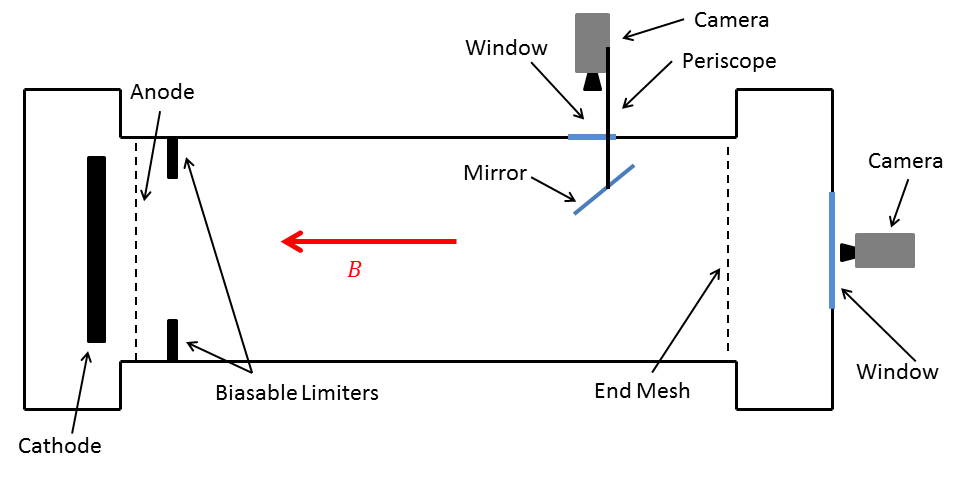
\includegraphics[width=8.5cm]{plot_of_LAPD}}
\caption{A basic cutaway of the setup of the LAPD; including the biasable limiters. The camera is shown in two different setups; first attached to the periscope (top) and second at the end of the LAPD (right).}
\label{fig:plot_of_LAPD}
\end{figure}


This experiment was conducted using the Large Plasma Device (LAPD). The LAPD is a cylindrically magnetized plasma device that is 18m long and 1m in diameter with a 54cm diameter barium-oxide coated nickel cathode. The cathode is pulsed at 1Hz to produce a 45eV electron beam which ionizes and heats the gas in the chamber. The magnetic field can be varied from 0.4kG to 2kG. For this experiment the magnetic field was set to 1kG, with a working gas of helium; the basic setup can be seen in Figure~\ref{fig:plot_of_LAPD}.

This study of flow via visable light imaging was only a small part of a larger study on flow and flow shear in the LAPD \citep{schaffner12, schaffner13}; this flow and flow shear was driven by biasing an adjustable circular limiter. The limiter is made up of four separate aluminum plates that can be inserted radially to set an opening diameter, functioning similarly to the iris of a camera lens. In this experiment the limiters were set to a radius of 26cm. This biasing creates a radially varying electric field and drives an azimuthal $E \times B$ flow and flow shear. The biasing and thus the azimuthal flow and shear were controlled by a capacitor bank that produced the voltage on the limiter plates. This setup enables fine control of the flow speed and shearing rate. When no voltage is applied to the limiter, the plasma spontaneously rotates in the ion diamagnetic direction (IDD).  When a voltage is applied to the limiter the plasma flow slows and when the voltage is approximately equal to that of the anode, the flow and the shear is zeroed out.  When the voltage on the limiters is greater than that of the anode, it produced a flow in the electron diamagnetic direction (EDD). The voltage on the power supply cannot be set lower than the floating potential of the plasma because the plasma will charge the capacitor banks. Thus, this limits the flow speed that can be obtained in the IDD, but larger flows can be driven in the EDD. In previous chamber wall biasing experiments on the LAPD \citep{Carter09}, it was only possible to obtain low and high flow states, with little to no control over the flow speeds.

\begin{figure}
\centerline{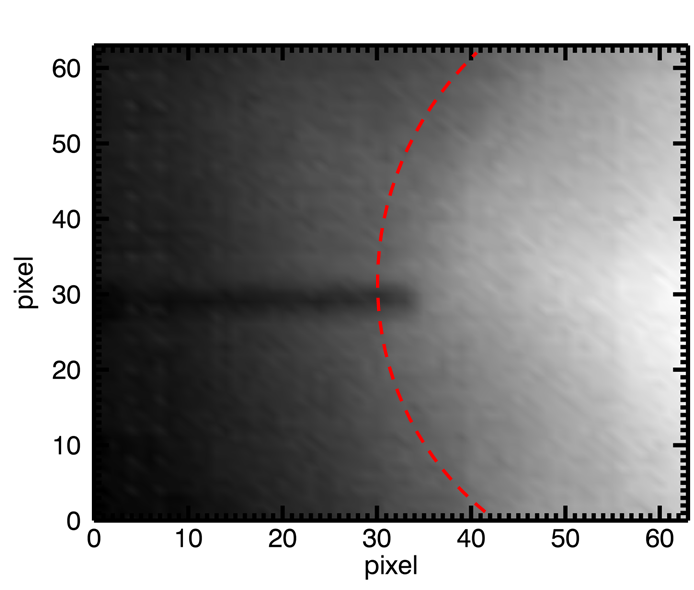
\includegraphics[width=8.5cm]{plot_movie_still}}
\caption{ This still from the fast framing camera shows a Langmuir probe inserted from the left and the tip in the center of the frame. The limiter edge can also be seen where the luminosity suddenly drops, and is highlighted by the dashed red curve which represents a radius of 26cm.}
\label{fig:plot_movie_still}
\end{figure}

Measurements of the visible light were made using a Phantom V7.3 fast framing camera. A 180mm Nikor lens was used without filters allowing the whole visible spectrum to be imaged. The aperture of the camera was chosen to be f/2.8 or f/4 so that it would limit the depth of field and thus limit the line integration effects of the imaging of plasma structures. There were two different camera setups used in this experiment, both of which can be seen in Figure~\ref{fig:plot_of_LAPD}.  For the first setup the camera was placed at the end of the LAPD and was aimed through the window at the cathode.  This view has primarily been used to qualitatively look at the plasma column due to image distortions and limited access to imaging straight down the radial edge of the column.  For all other data taken the camera was placed on a specially designed periscope, which enabled a better line of sight to image the edge region of the LAPD while maintaining a straight coaxial line of sight down the device and down the field aligned plasma structures. The camera is attached to the periscope pointing radially inward looking through a window on the side of the LAPD. Inside of the LAPD there is a mirror attached to the periscope that can be adjusted through ninety degrees. The mirror is aligned to a forty-five degree angle by placing the center of the mirror at the same radial position as two axially separated probes; then the mirror is rotated until the probe tip nearest to the mirror overlaps the farther probe tip in the center of the field of view of the camera. The mirror and camera separation can be fixed, allowing for movement of the periscope setup to different radial positions without the need for adjusting focus.  The periscope was placed a few meters from the end of the LAPD and was grounded to the chamber wall.  This setup is assumed to cause only a small perturbation in the plasma due to the long parallel wavelengths observed in the LAPD.  For the correlations performed with the Langmuir probe, the camera took data using a 64 by 128 pixel frame with a frame rate of 100kfps and a resolution of about 1mm per pixel.  All the other data presented here was taken using a 128 by 128 pixel frame and a frame rate of approximately 85kfps, an exposure of $2 \mu s$ and a linear resolution of approximately 1mm per pixel.  The data was taken over a radial range from about $17cm$ to $30cm$.
 
Multiple probes were used to study the effects of flow and flow shear on particle transport \citep{schaffner12, schaffner13}; these diagnostics were also used to compare with the fast framing camera. Some of these probes included: a six sided Mach probe was used to measure the velocity of the plasma, a swept Langmuir probel, and a multi-tipped flux probe. Measurements of ion saturation current $(I_{sat})$, temperature $(T_e)$, and floating potential $(V_f)$ were made with a triple probe. From these we can estimate the density $(n_e)$ from:

\begin{equation} I_{sat}=n_e T_e^{1/2}
\label{eq:one}
\end{equation}

In the next section we will discuss comparing these measurements to the measurements of luminosity made by the camera.


\section{Correlation and Comparison}


\begin{figure}
\centerline{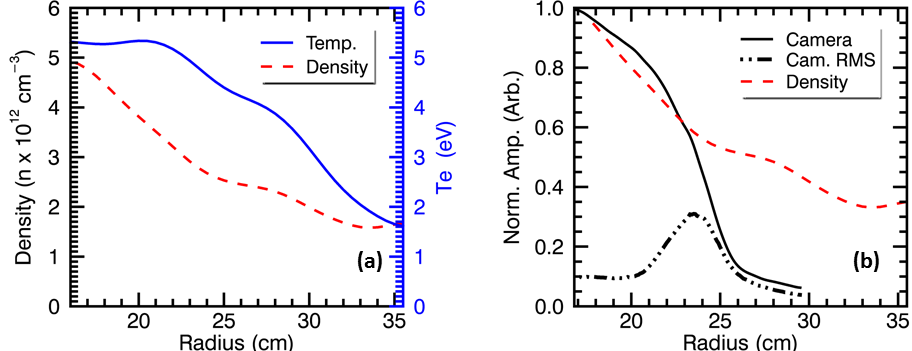
\includegraphics[width=8.5cm]{plot_dens_lum_temp_4_0V}}
\caption{  (a) Radial profiles of both the density (dashed red) and temperature (blue) measured by a swept Langmuir probe.  (b) A comparison of the normalized camera intensity (black), the normalized density (dashed red)  and the camera intensity RMS fluctuations (dash-dot black). }
\label{fig:plot_dens_lum_temp_4_0V}
\end{figure}

The primary source of light produced in the LAPD comes from the neutral helium line; which is primarily caused by plasma electron and neutral helium collisions. The intensity of light emitted has the form $I \propto n_0f(n_e, T_e)$, where $n_0$ is neutral density and $f(n_e, T_e)$ is some unknown function of plasma density and temperature. In the LAPD the neutral density does not change much over time scale of the experiment, so $n_0$ can be taken to be a constant in space and time \citep{maggs07}. Thus, leaving the intensity in this form $I \propto f(n_e, T_e)$.  Other experiments \citep{antar07, light13} have rather uniform temperature profiles across their plasma columns with small fluctuations in temperature compared to density; both of these are not the case in the LAPD plasma. One can see in Figure~\ref{fig:plot_dens_lum_temp_4_0V}a that both the time averaged temperature and density profiles drop off over the range that is being imaged.  In Figure~\ref{fig:plot_dens_lum_temp_4_0V}b the time averaged normalized intensity of the camera follows the density fairly well until about 24cm, when it drops suddenly; probably due to the drop in temperature.  Part of this problem can be resolved by the fact that the temperature and density fluctuations are in phase with each other. Taking this into account the assumption is made that the light that is detected is approximately proportional plasma density, just as many make the same assumption when looking at an $I_{sat}$ signal. As for the drop off in the camera intensity at large radii, it will be seen later that this limits the radial distance at which the camera is an effective plasma diagnostic; and we will simply ignore these regions of low luminosity.

\begin{figure}
\centerline{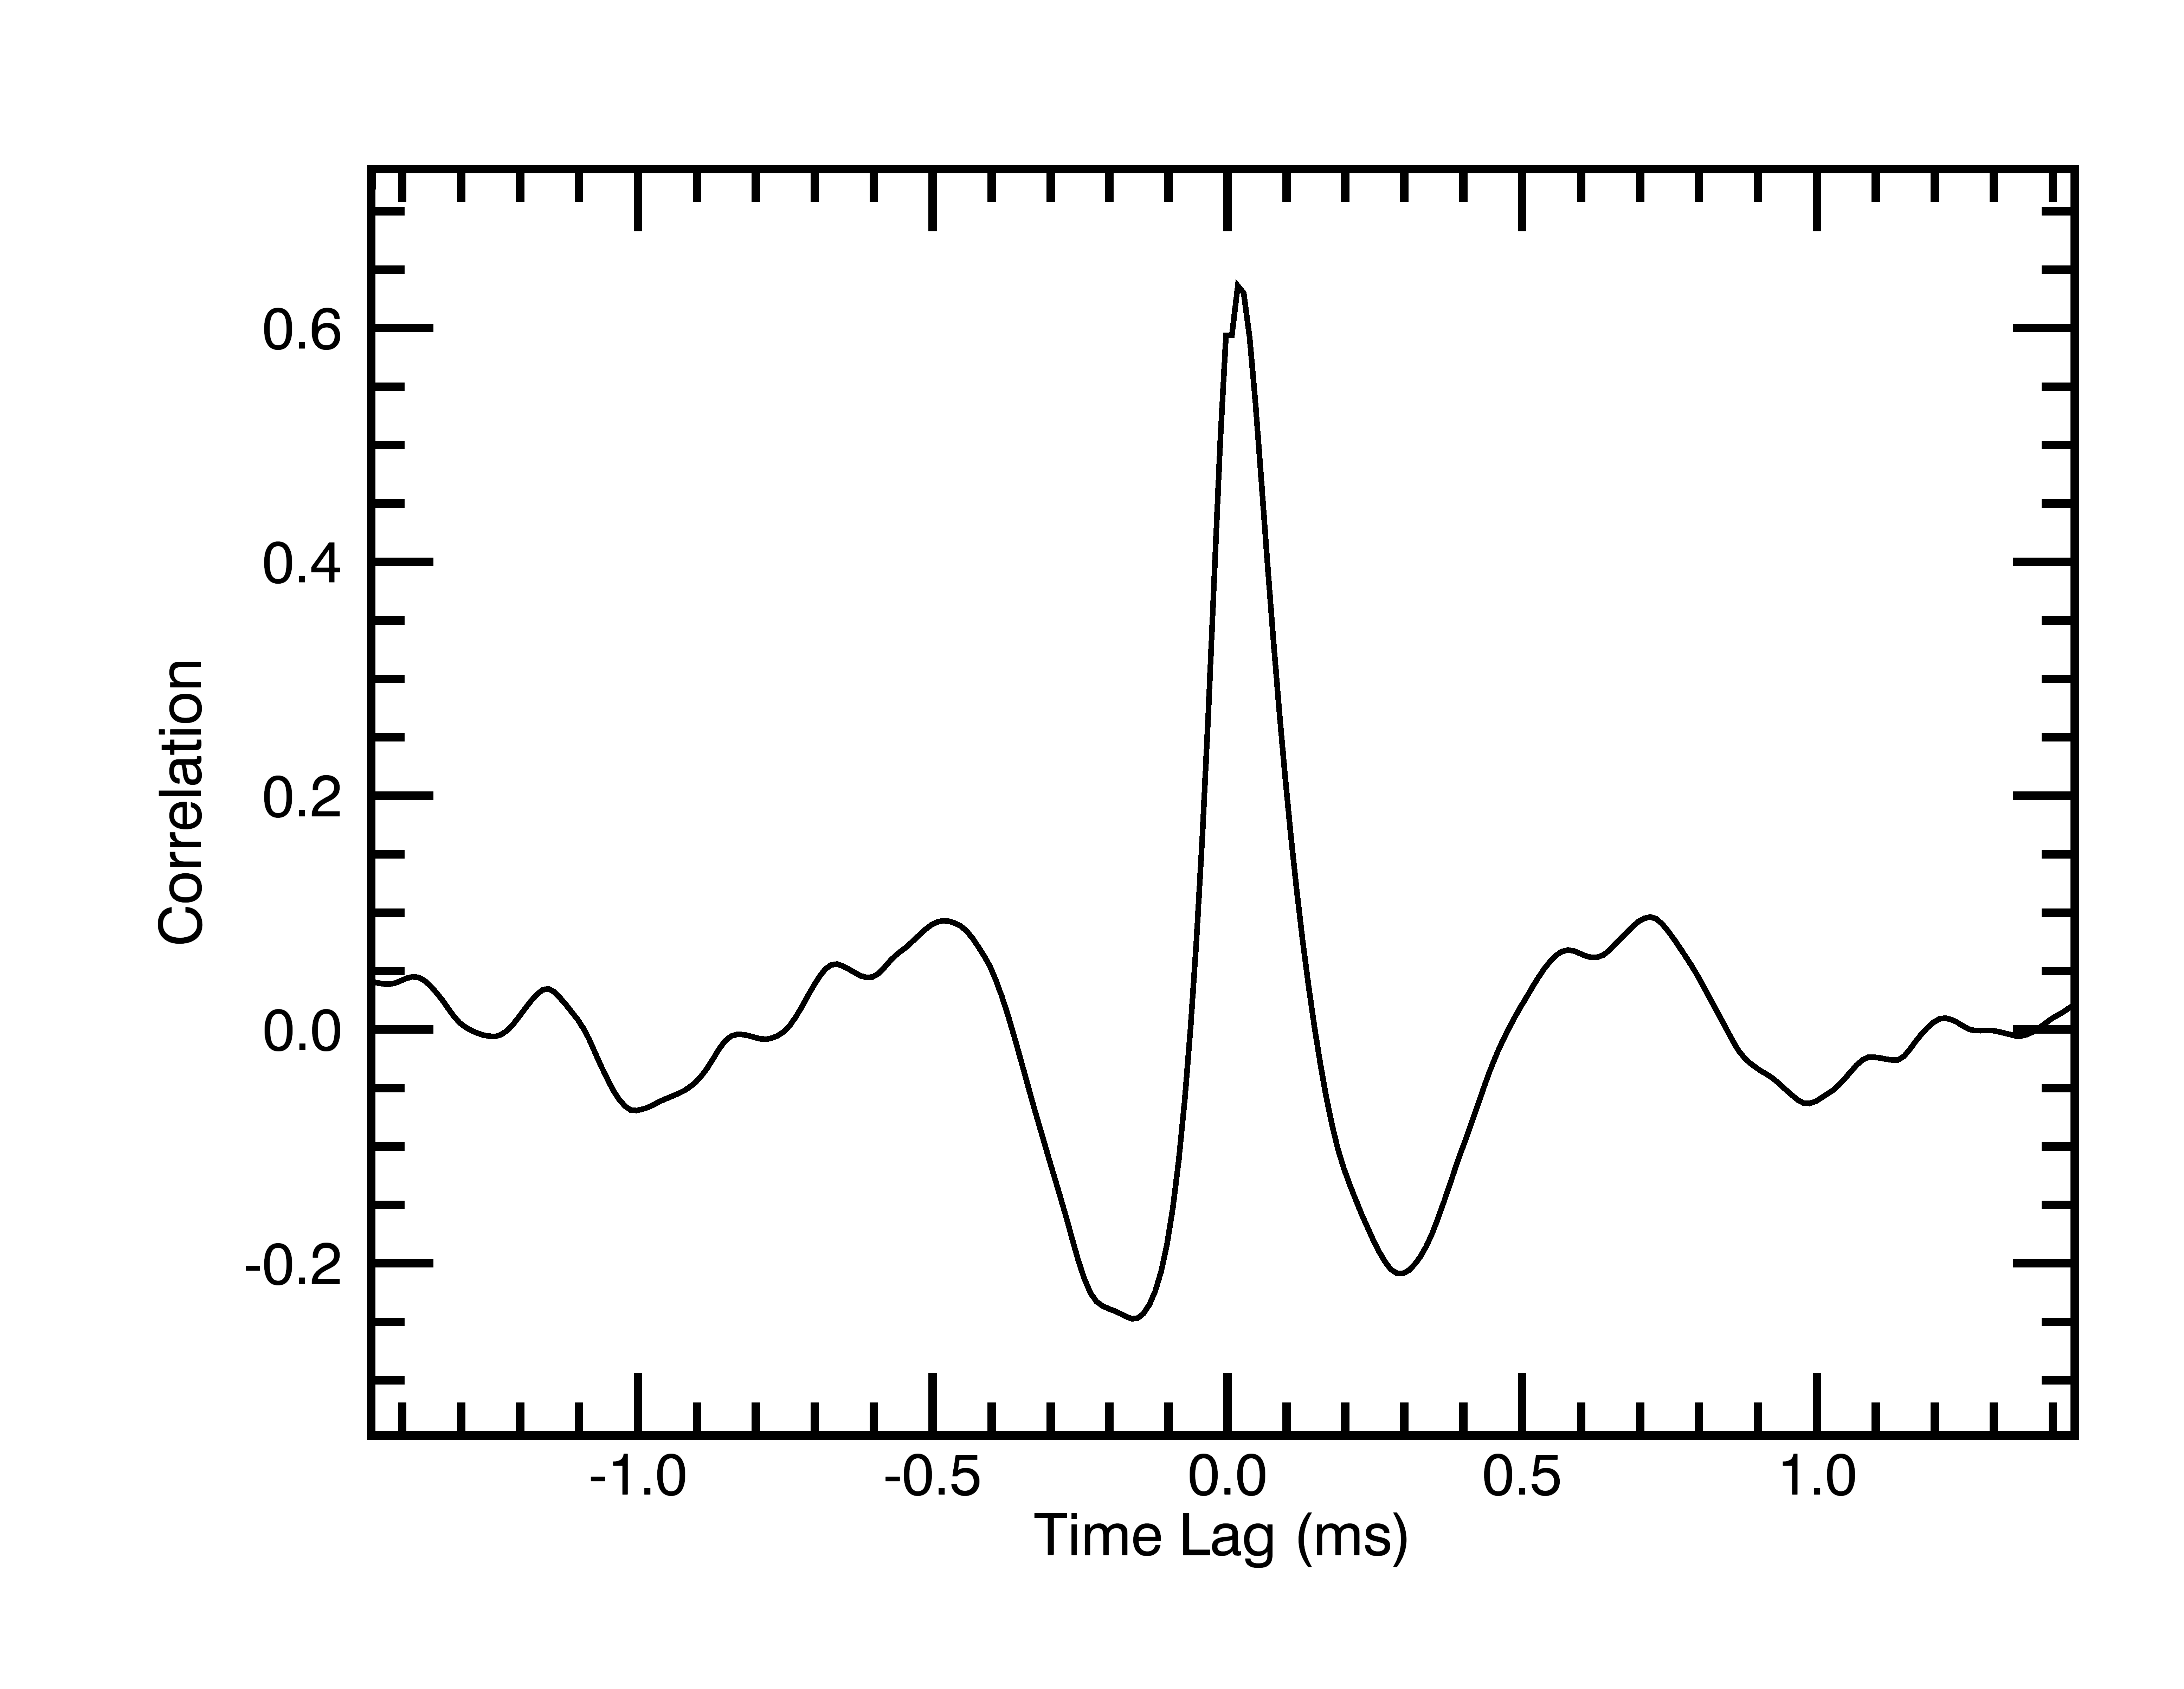
\includegraphics[width=8.5cm]{plot_Camera_probe_correlation_23cm_0V}}
\caption{ Cross correlation of luminosity and $I_{sat}$ signals for an unbiased case with flow in the IDD.  A high peak correlation of greater than 0.6 is seen. }
\label{fig:plot_Camera_probe_correlation_23cm_0V}
\end{figure}

To establish a physical link between the luminosity measured by the camera and the plasma parameters measured by a Langmuir probe, the correlation between two simultaneous signals was taken. The probe was placed in the LAPD at 23cm radially from the center of the plasma column, just inside of the limiters edge which in this case were situated at approximately 26cm. The limiter was also set to an unbiased state, letting the plasma flow in the IDD. The camera was focused on the probe tip approximately 10m from the camera. Data was simultaneously taken by both the camera and the probe. Forty separate plasma discharges were used to create an ensemble in this comparison.  The ion saturation current from the probe was taken as a proxy for the plasma density and was compared to the camera luminosity taken from a single pixel next to the probe in the camera frame, an example frame can be seen in Figure~\ref{fig:plot_movie_still}. Next, the $(I_{sat})$ data was down sampled to match the frame rate of the camera, and the mean was subtracted from both time traces leaving only the fluctuations. The cross correlation of the two signals is plotted in Figure~\ref{fig:plot_Camera_probe_correlation_23cm_0V}. Both signals are well correlated with the peak exceeding 0.6 and they are nearly at a time delay of zero. The offset of the peak of the cross correlation is on the order of the frame rate of the camera. Multiple tests were conducted at different biases causing flow in both the EDD and IDD and different radii from the center of the plasma; all with high peak correlations ranging from about 0.5 to 0.7, similar to the one shown here.

\begin{figure}
\centerline{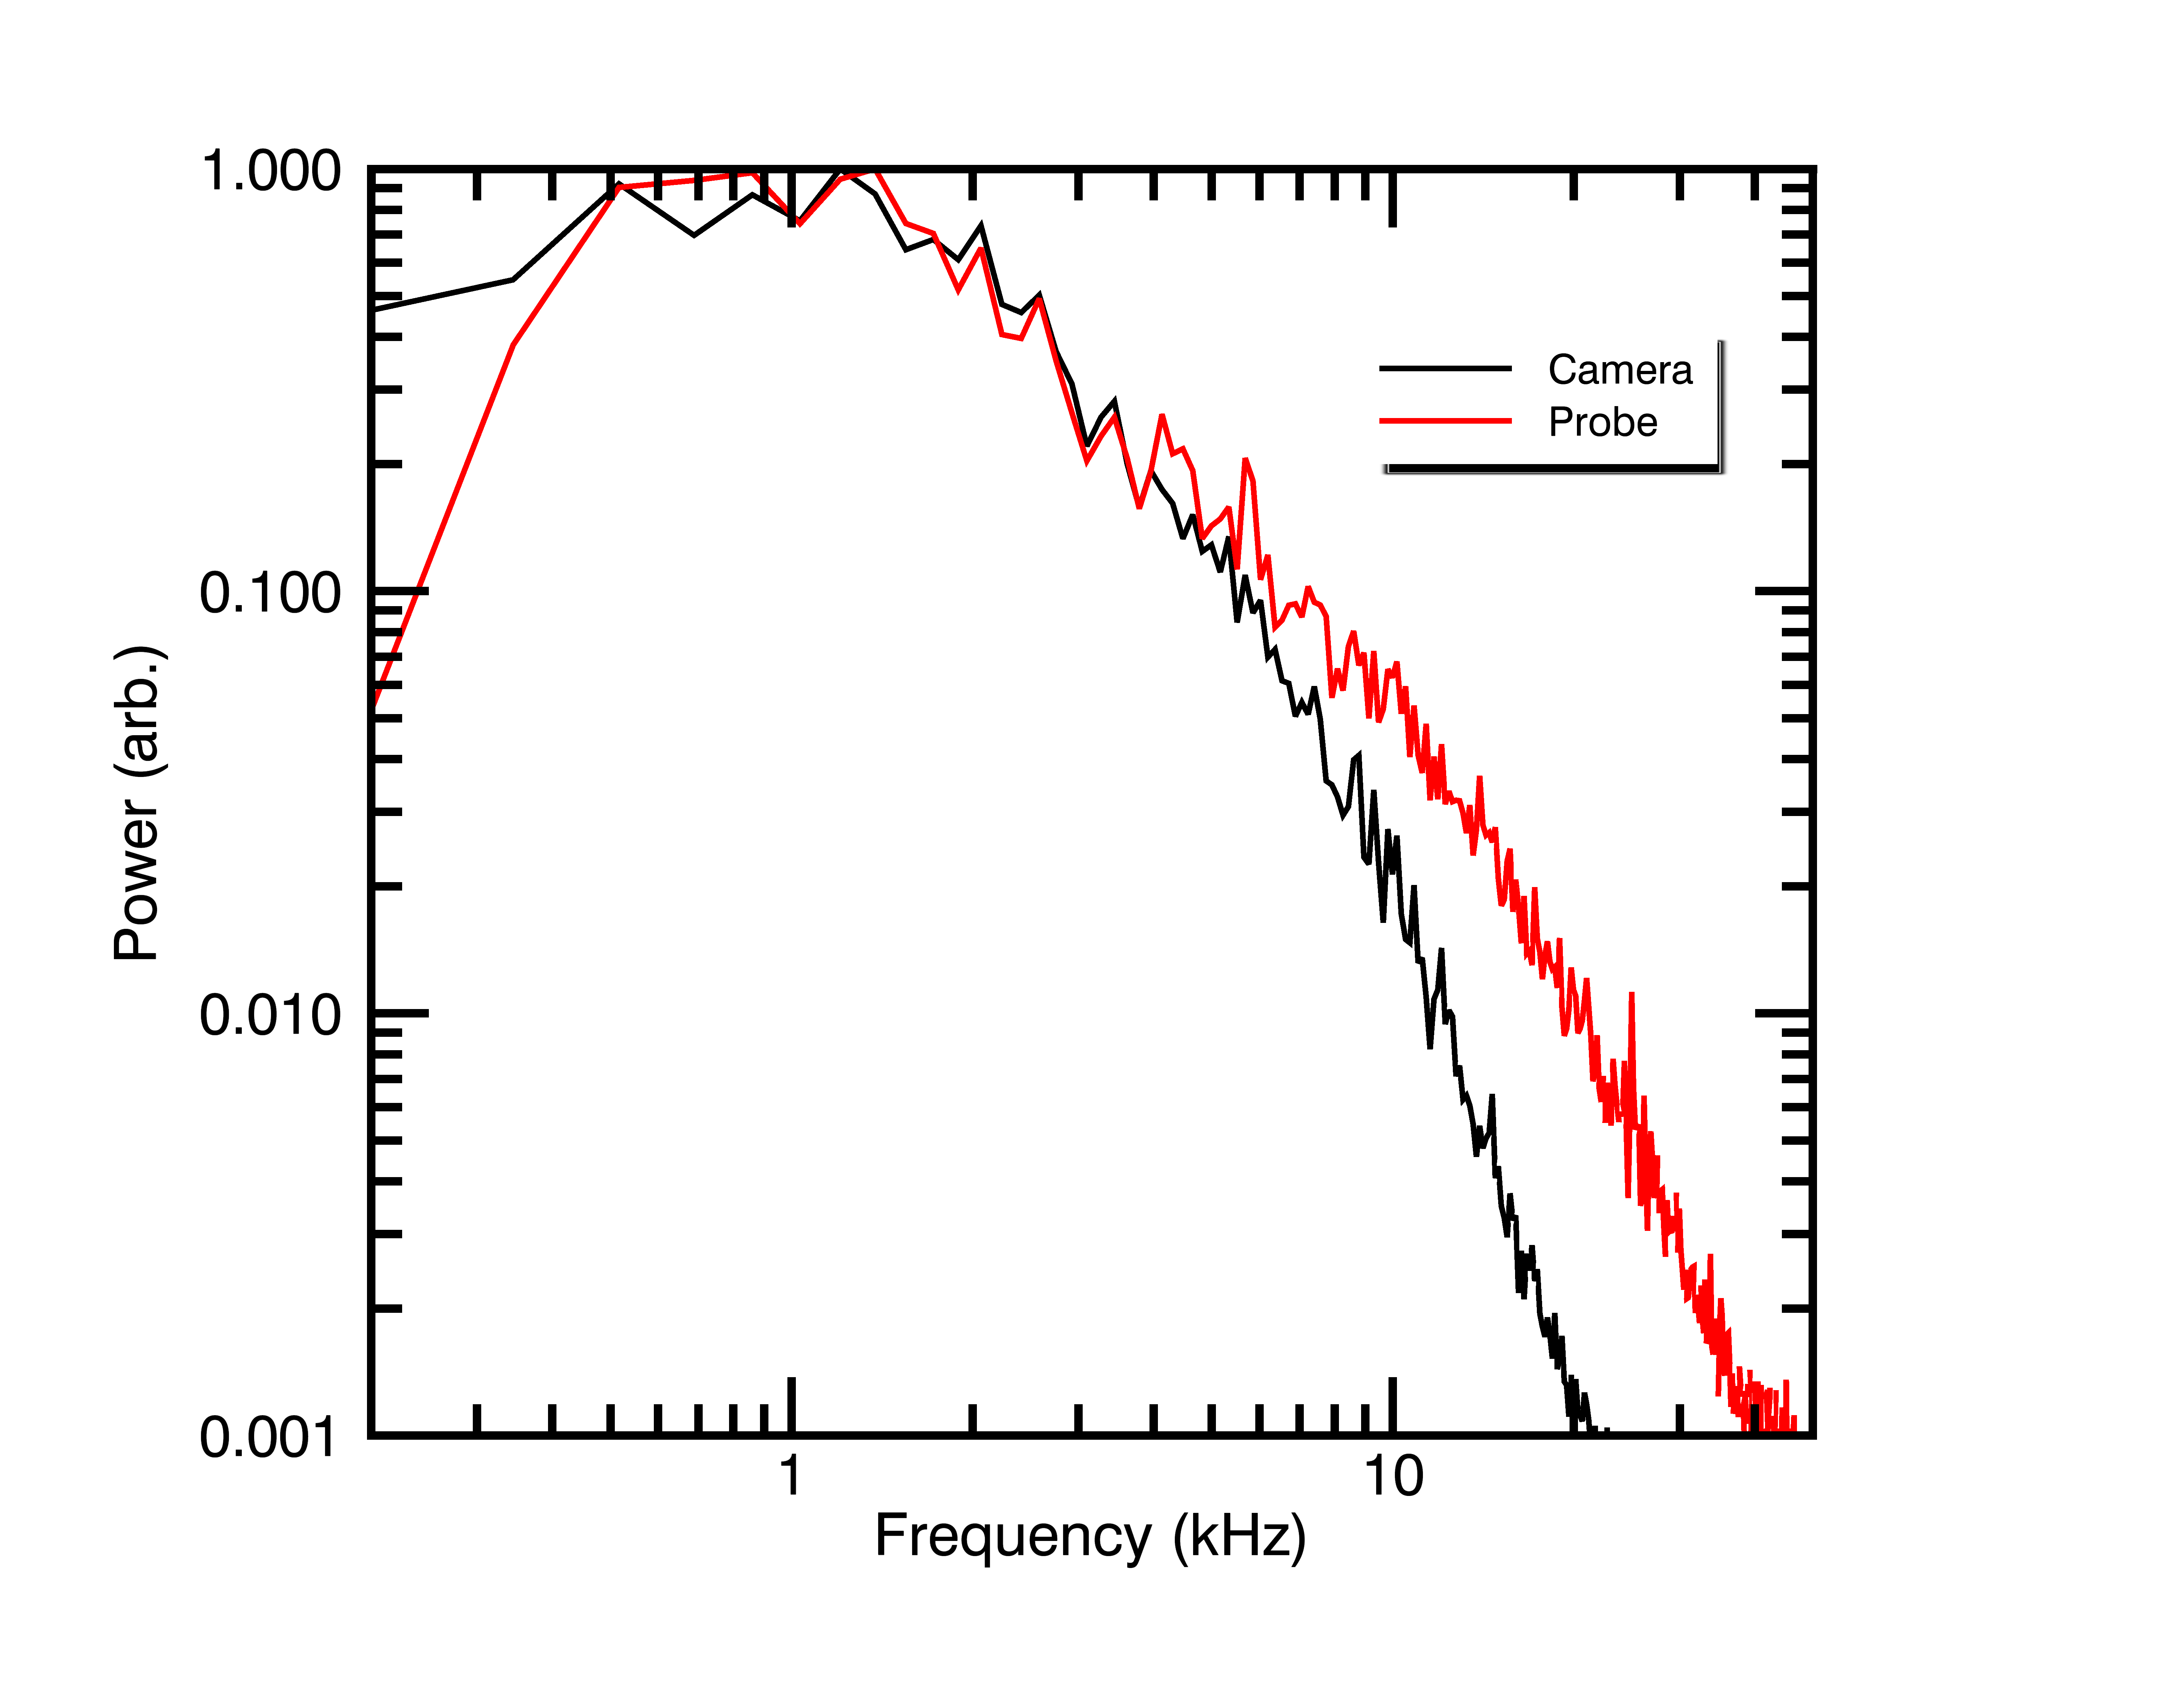
\includegraphics[width=8.5cm]{plot_Freq_spectra_cam_probe_bias_0V_23cm}}
\caption{The normalized power spectrum of the probe (red) and camera (black) signals; showing good agreement across most of the frequency spectrum. }
\label{fig:plot_Freq_spectra_cam_probe_bias_0V_23cm}
\end{figure}

Figure~\ref{fig:plot_Freq_spectra_cam_probe_bias_0V_23cm} shows the normalized auto power spectrum of the camera and probe signals for the unbiased case. This is the auto power spectrum of both the $(I_{sat})$ signal and of the luminosity signal from the pixel near the probe in the camera frame. Just by visual inspection, the two signals appear to be in good agreement up to about 6kHz.  This departure from agreement at high frequency is most likely caused by line integration effects from imaging the plasma. This effect essentially lowers the spatial resolution of the camera. 


\begin{figure}
\centerline{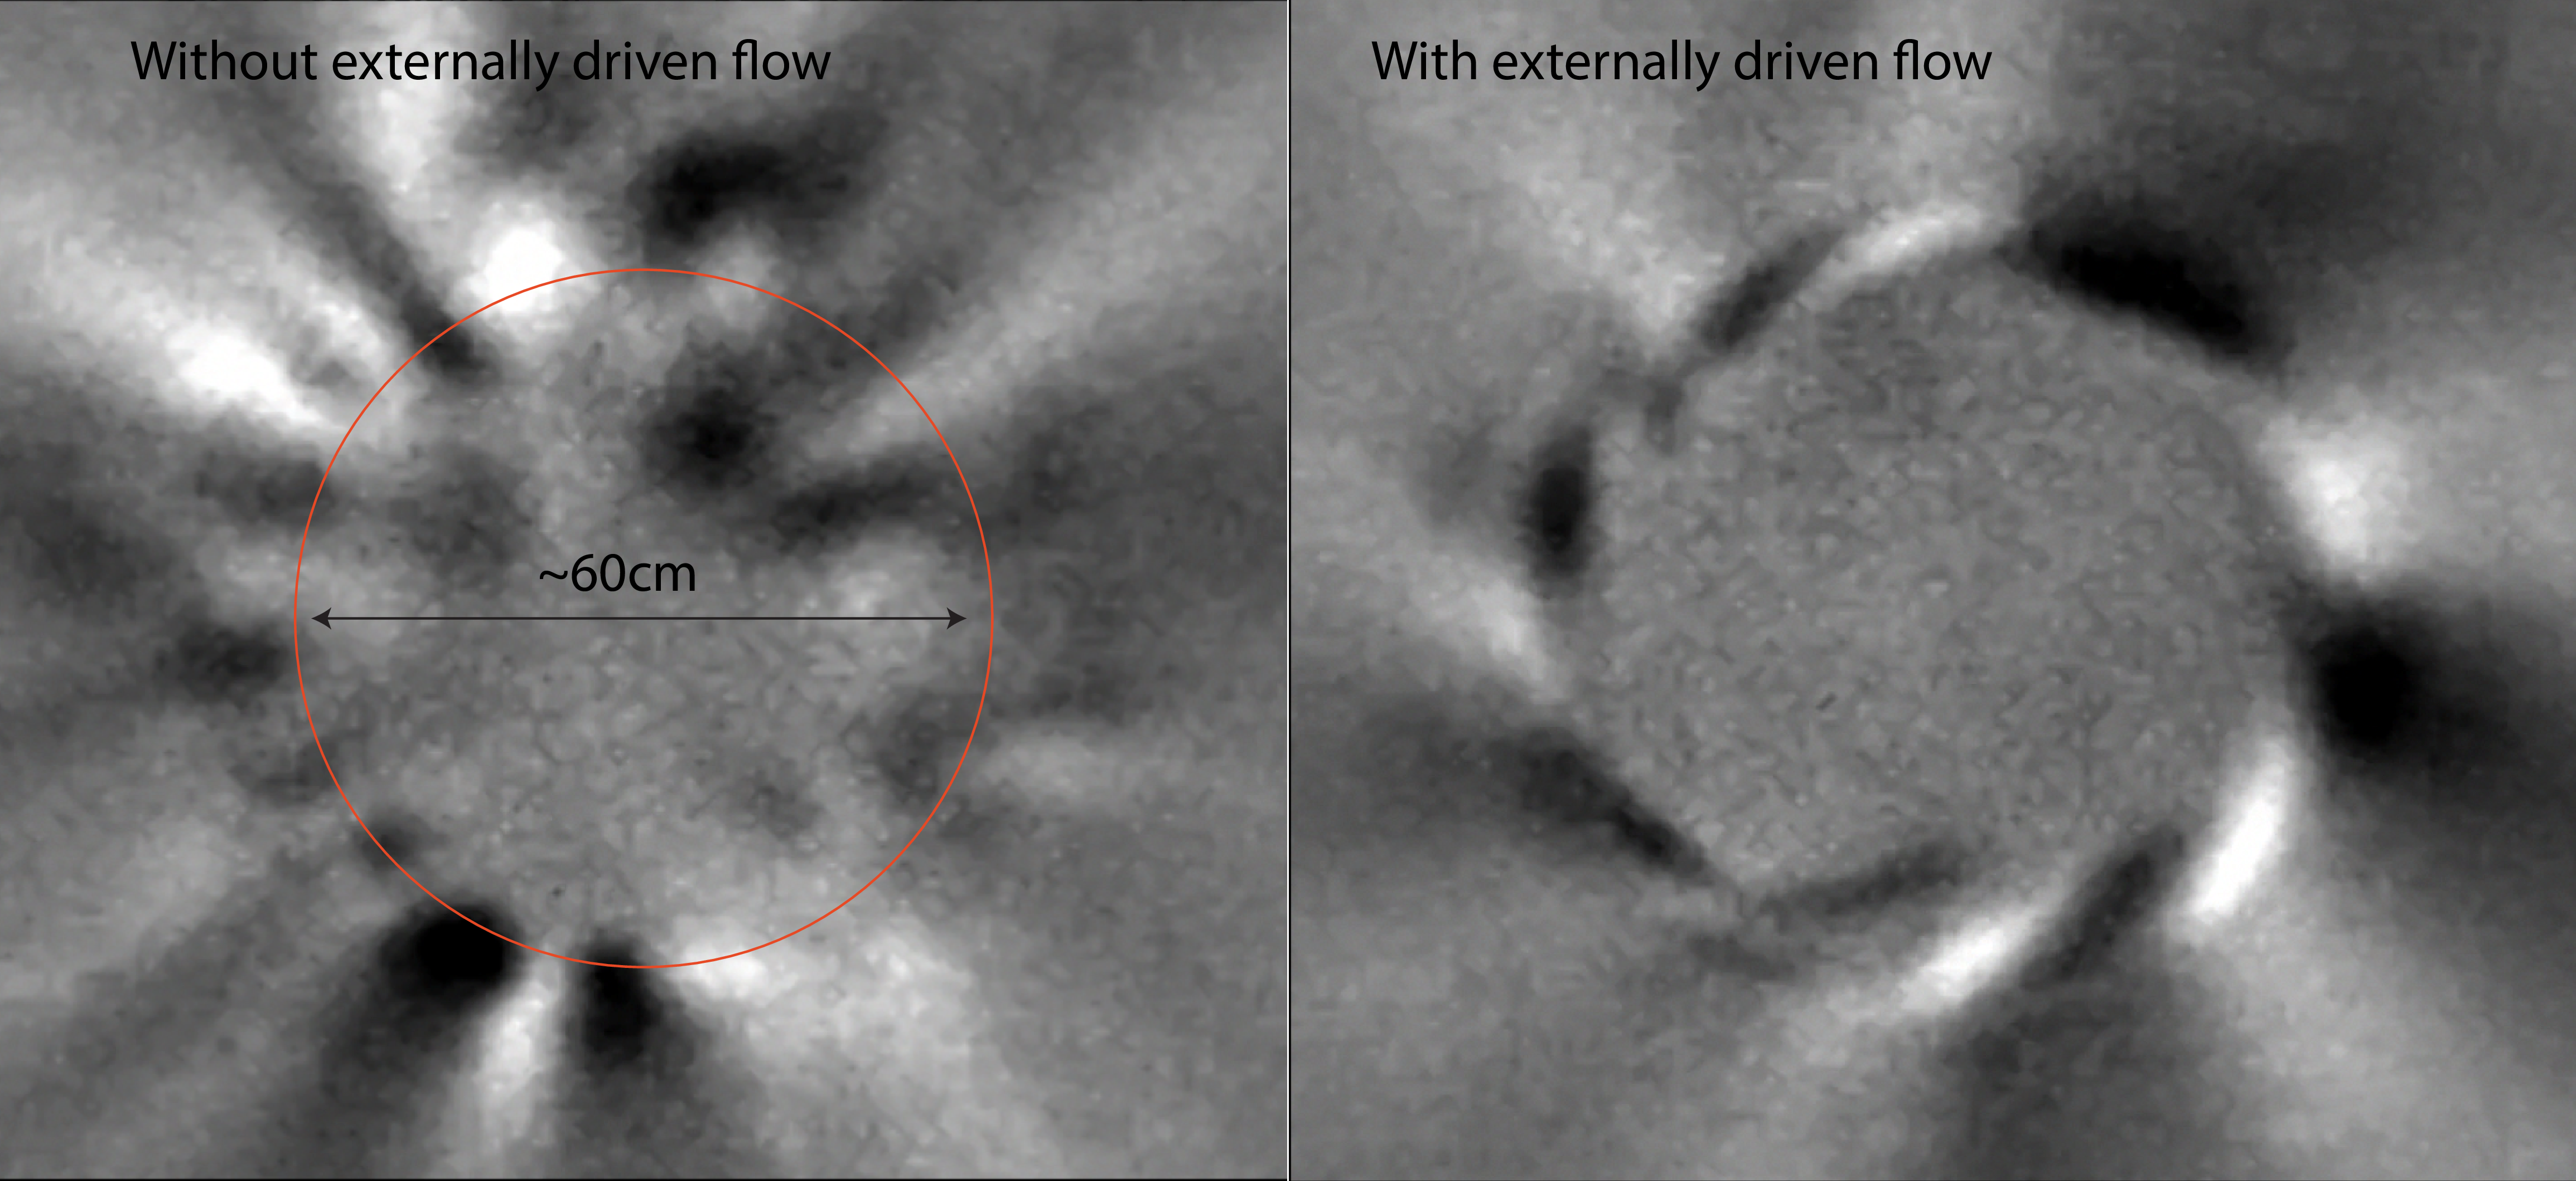
\includegraphics[width=8.5cm]{plot_camera_images_flow}}
\caption{Two images from the fast framing camera, taken through the end window of the LAPD showing the full plasma column. Left: showing the plasma in its unbiased rotation state in the IDD direction.  The approximate location of the limiter edge can be seen in red.  Right: shows the plasma with a high bias applied to the limeters causing high flow and flow shear near the limiter edge.  Note, this camera view was not used due to the large amount of optical distortions seen near the edges of the field of view.}
\label{fig:plot_camera_images_flow}
\end{figure}




\begin{figure}
\centerline{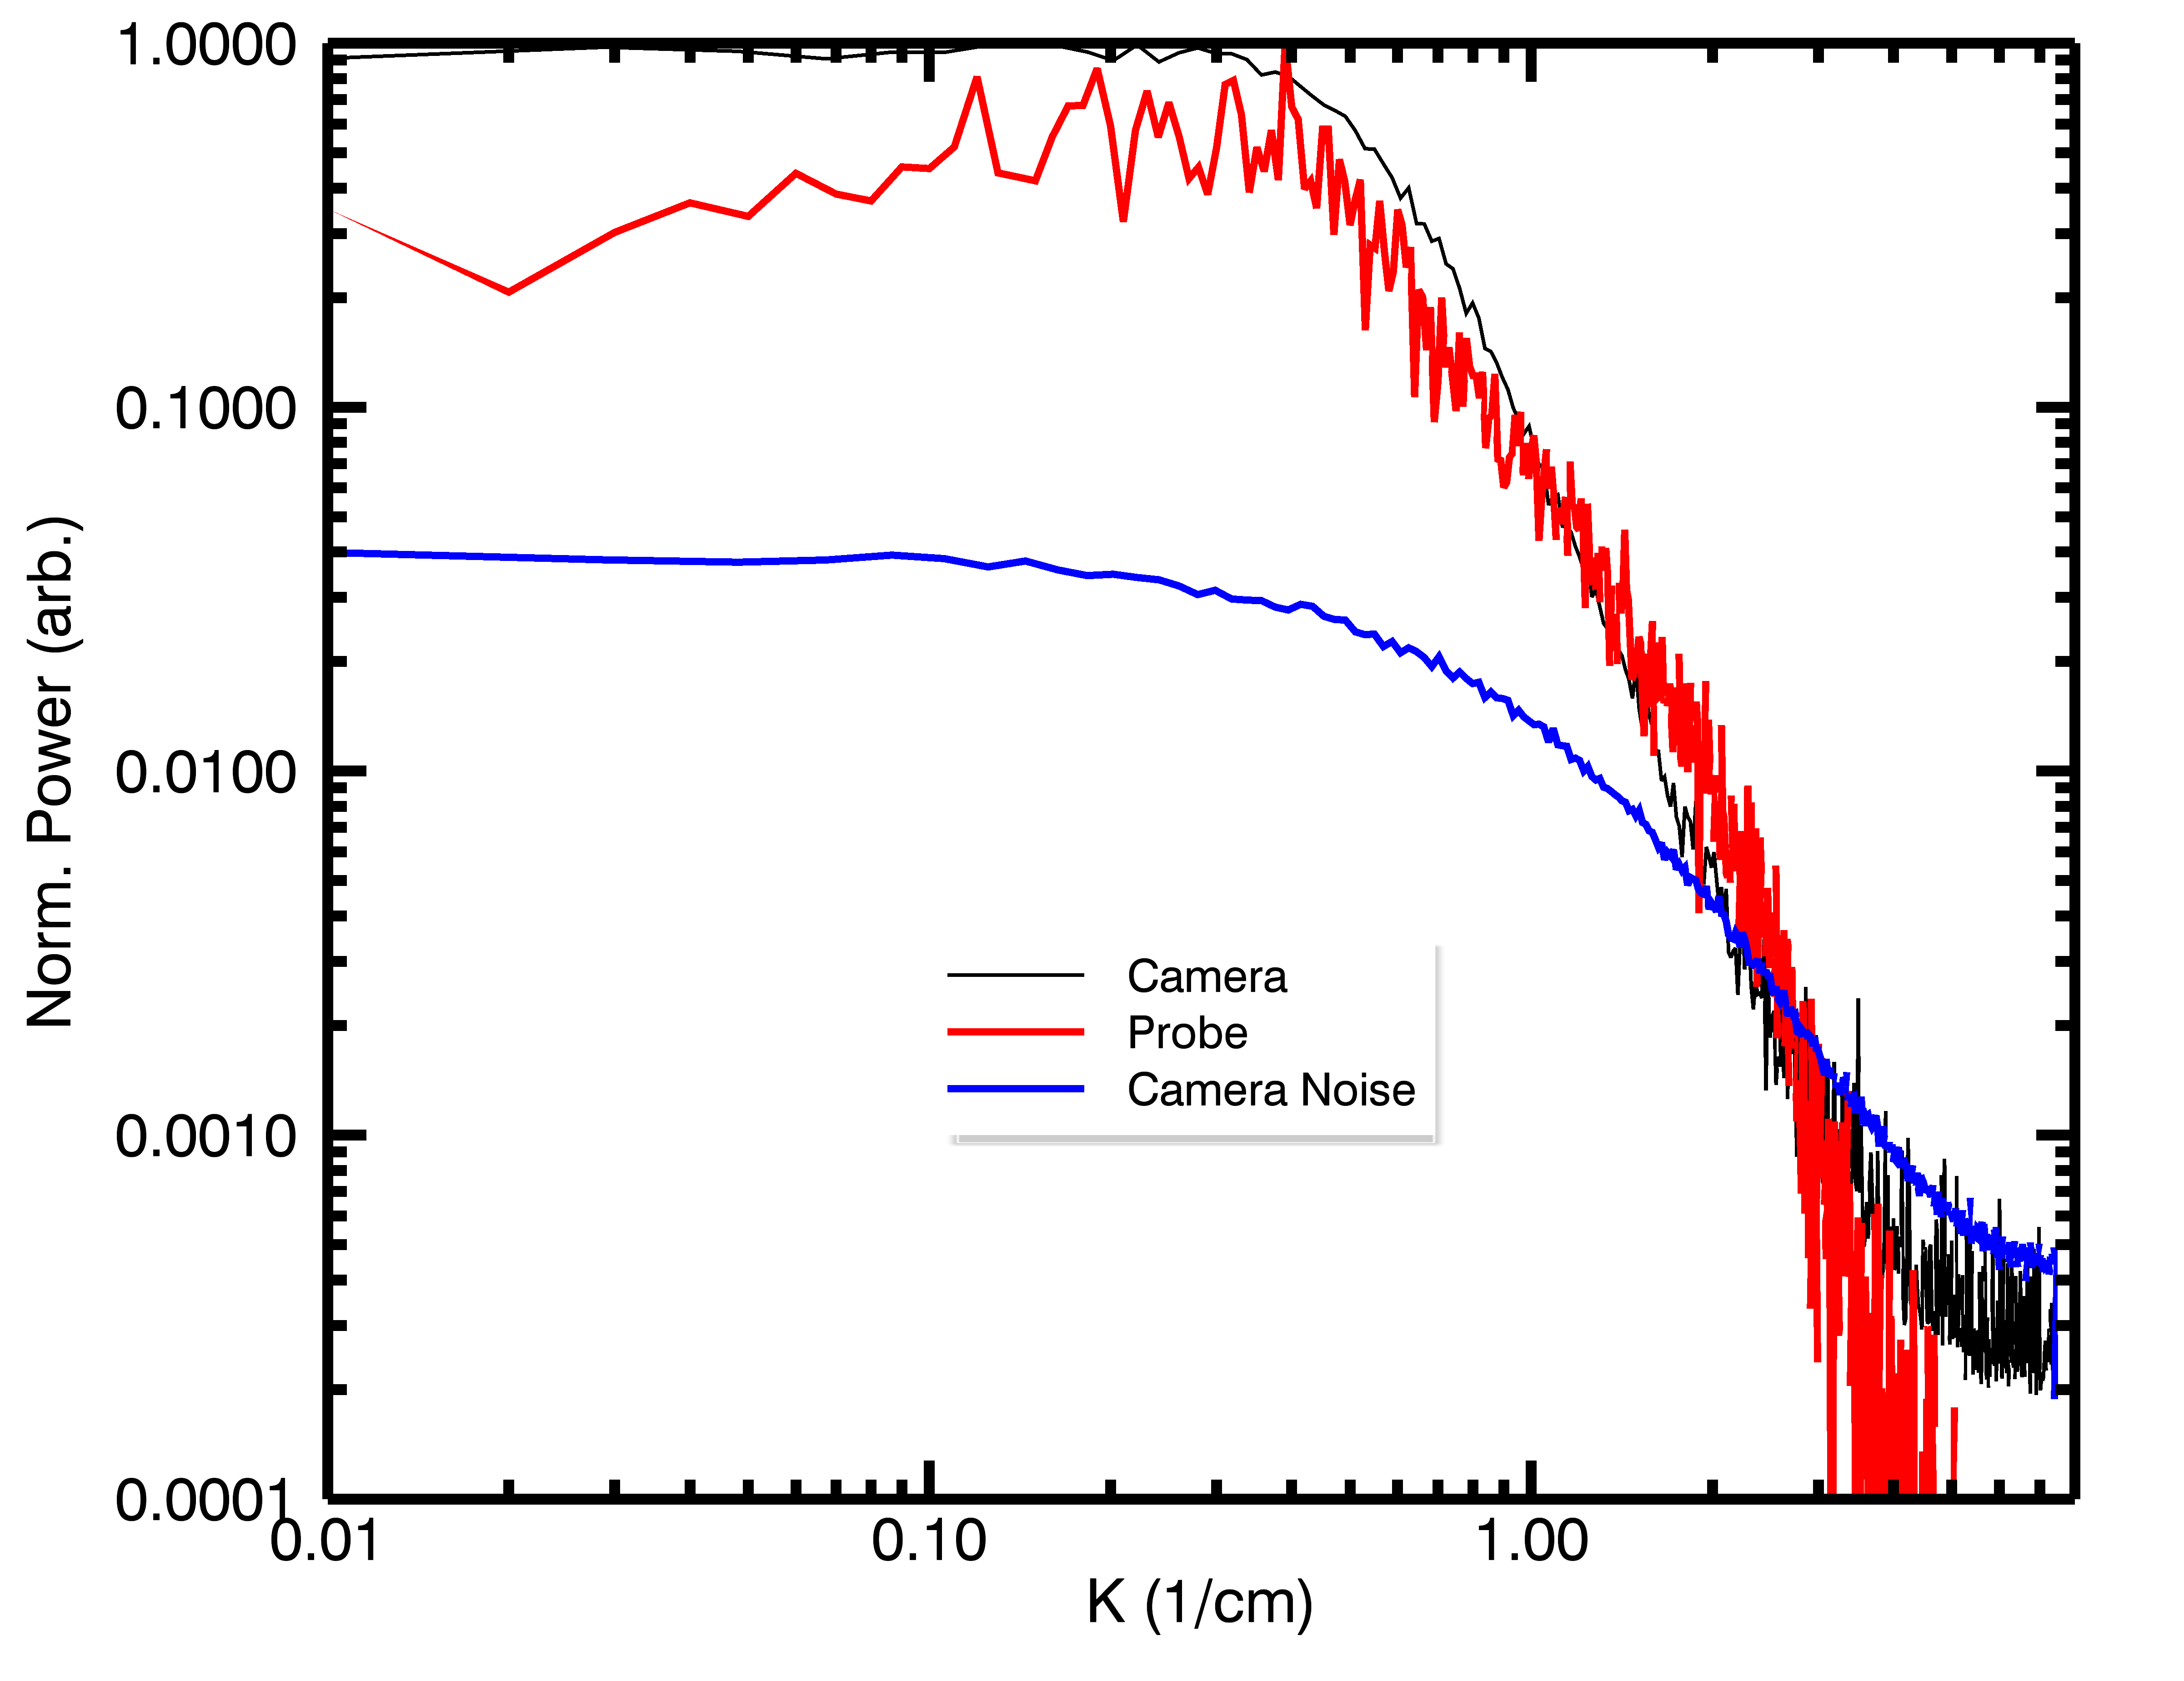
\includegraphics[width=8.5cm]{plot_k_spectra}}
\caption{ The K-spectrum is plotted from both camera pixel pairs (black) and probe pairs (red). Both diagnostics are in good agreement in values of K less than about 2. This is where the camera drops below the noise floor (blue). }
\label{fig:plot_k_spectra}
\end{figure}


The biggest advantage of using a fast framing camera can be seen in Figure~\ref{fig:plot_camera_images_flow}, where the spatial structures can be seen in a single plasma discharge. Here, two different movie stills are shown at different times in the experiment.  First, the left image shows the plasma in an unbiased state before the bias is turned on.  To the right, a bias of 150V has been applied and causes a large flow in the EDD and flow shear.  It is easily seen how the biasing has modified the plasma structure from the unbiased to biased state.  The plasma structures have been tilted and elongated in the azimuthal direction and has changed the dominant mode number.  These movies were taken at the end of the LAPD with a wide field of view lens. One can also see optical distortions and line integration effects develop quickly as you move from the center of the field of view; making it difficult to accurately estimate the size and velocity of these structures. These distortions and other limitations led to the development of the camera periscope system used for most of the data in this paper.

Lastly, the K-spectrum was calculated using both the camera and a probe. The method \citep{beall82} used here is calculated using pairs of probes separated by a small distance. In the case of the camera, pixel pairs were chosen that had a similar linear separation distance as the probe pairs. As you can see in Figure~\ref{fig:plot_k_spectra} the camera and probe agree nicely when the camera data is above its noise floor.
 


\section{Wavelet Velocity}

This section discusses a wavelet based method \citep{chaston10} for calculating instantaneous velocity fields from camera data. First a brief explanation is presented on how the method is performed and how it works. This is followed by an application of the wavelet method to BOUT$++$ simulation data. These results will then be compared to the velocity calculated from the $E \times B$ flow from the simulation. Finally, the method is applied to real camera data taken on the LAPD and compared to results of swept Langmuir probe measurements of the velocity.



\subsection{Wavelet Method}

To calculate instantaneous velocity fields from the fast camera a wavelet based method was used. First, a time average is subtracted from the data set at each pixel, thus leaving just the luminosity fluctuations. A 1D continuous complex wavelet transform is performed on each camera still in the time series. In this case the wavelet used was of type Paul and sixth order but the Morlet wavelet has also been used with similar results. This was done in both the vertical and horizontal directions of the frames over all the pixels. Where the vertical and horizontal transforms provide the vertical and horizontal velocity components respectively. The complex wavelet transform gives both intensity and phase at every pixel and wavelet scale $(\lambda_s)$. The change in phase angle $(\Delta\phi)$ between each successive frame is calculated. Dividing this by $2\pi$ and multiplying by its respective wavelet scale will give a spatial shift of the luminosity. Given that the luminosity is a measurement of density it can be said that this is a shift in the plasma density. Knowing the time step between frames, the velocity can be calculated by the following:

\begin{equation} v_s=\frac{\Delta\phi}{2\upi}\frac{1}{\Delta t}\lambda_s
\label{eq:two}
\end{equation}
Where $\Delta t$ is the time step between each frame. This will give us velocities as a function of the pixel location and wavelet scale. Next, the wavelet auto-power spectrum $(\vert W(s) \vert^2)$ is used to calculate a weighted average of the velocity over all the wavelet scales. The final result is an instantaneous velocity vector at each pixel given by:

 \begin{equation} v=\frac{\sum\vert W(s)\vert^2 v_s} {\sum \vert W(s) \vert^2}
\label{eq:three}
\end{equation}


\subsection{Application to BOUT++ Simulation}

\begin{figure}
\centerline{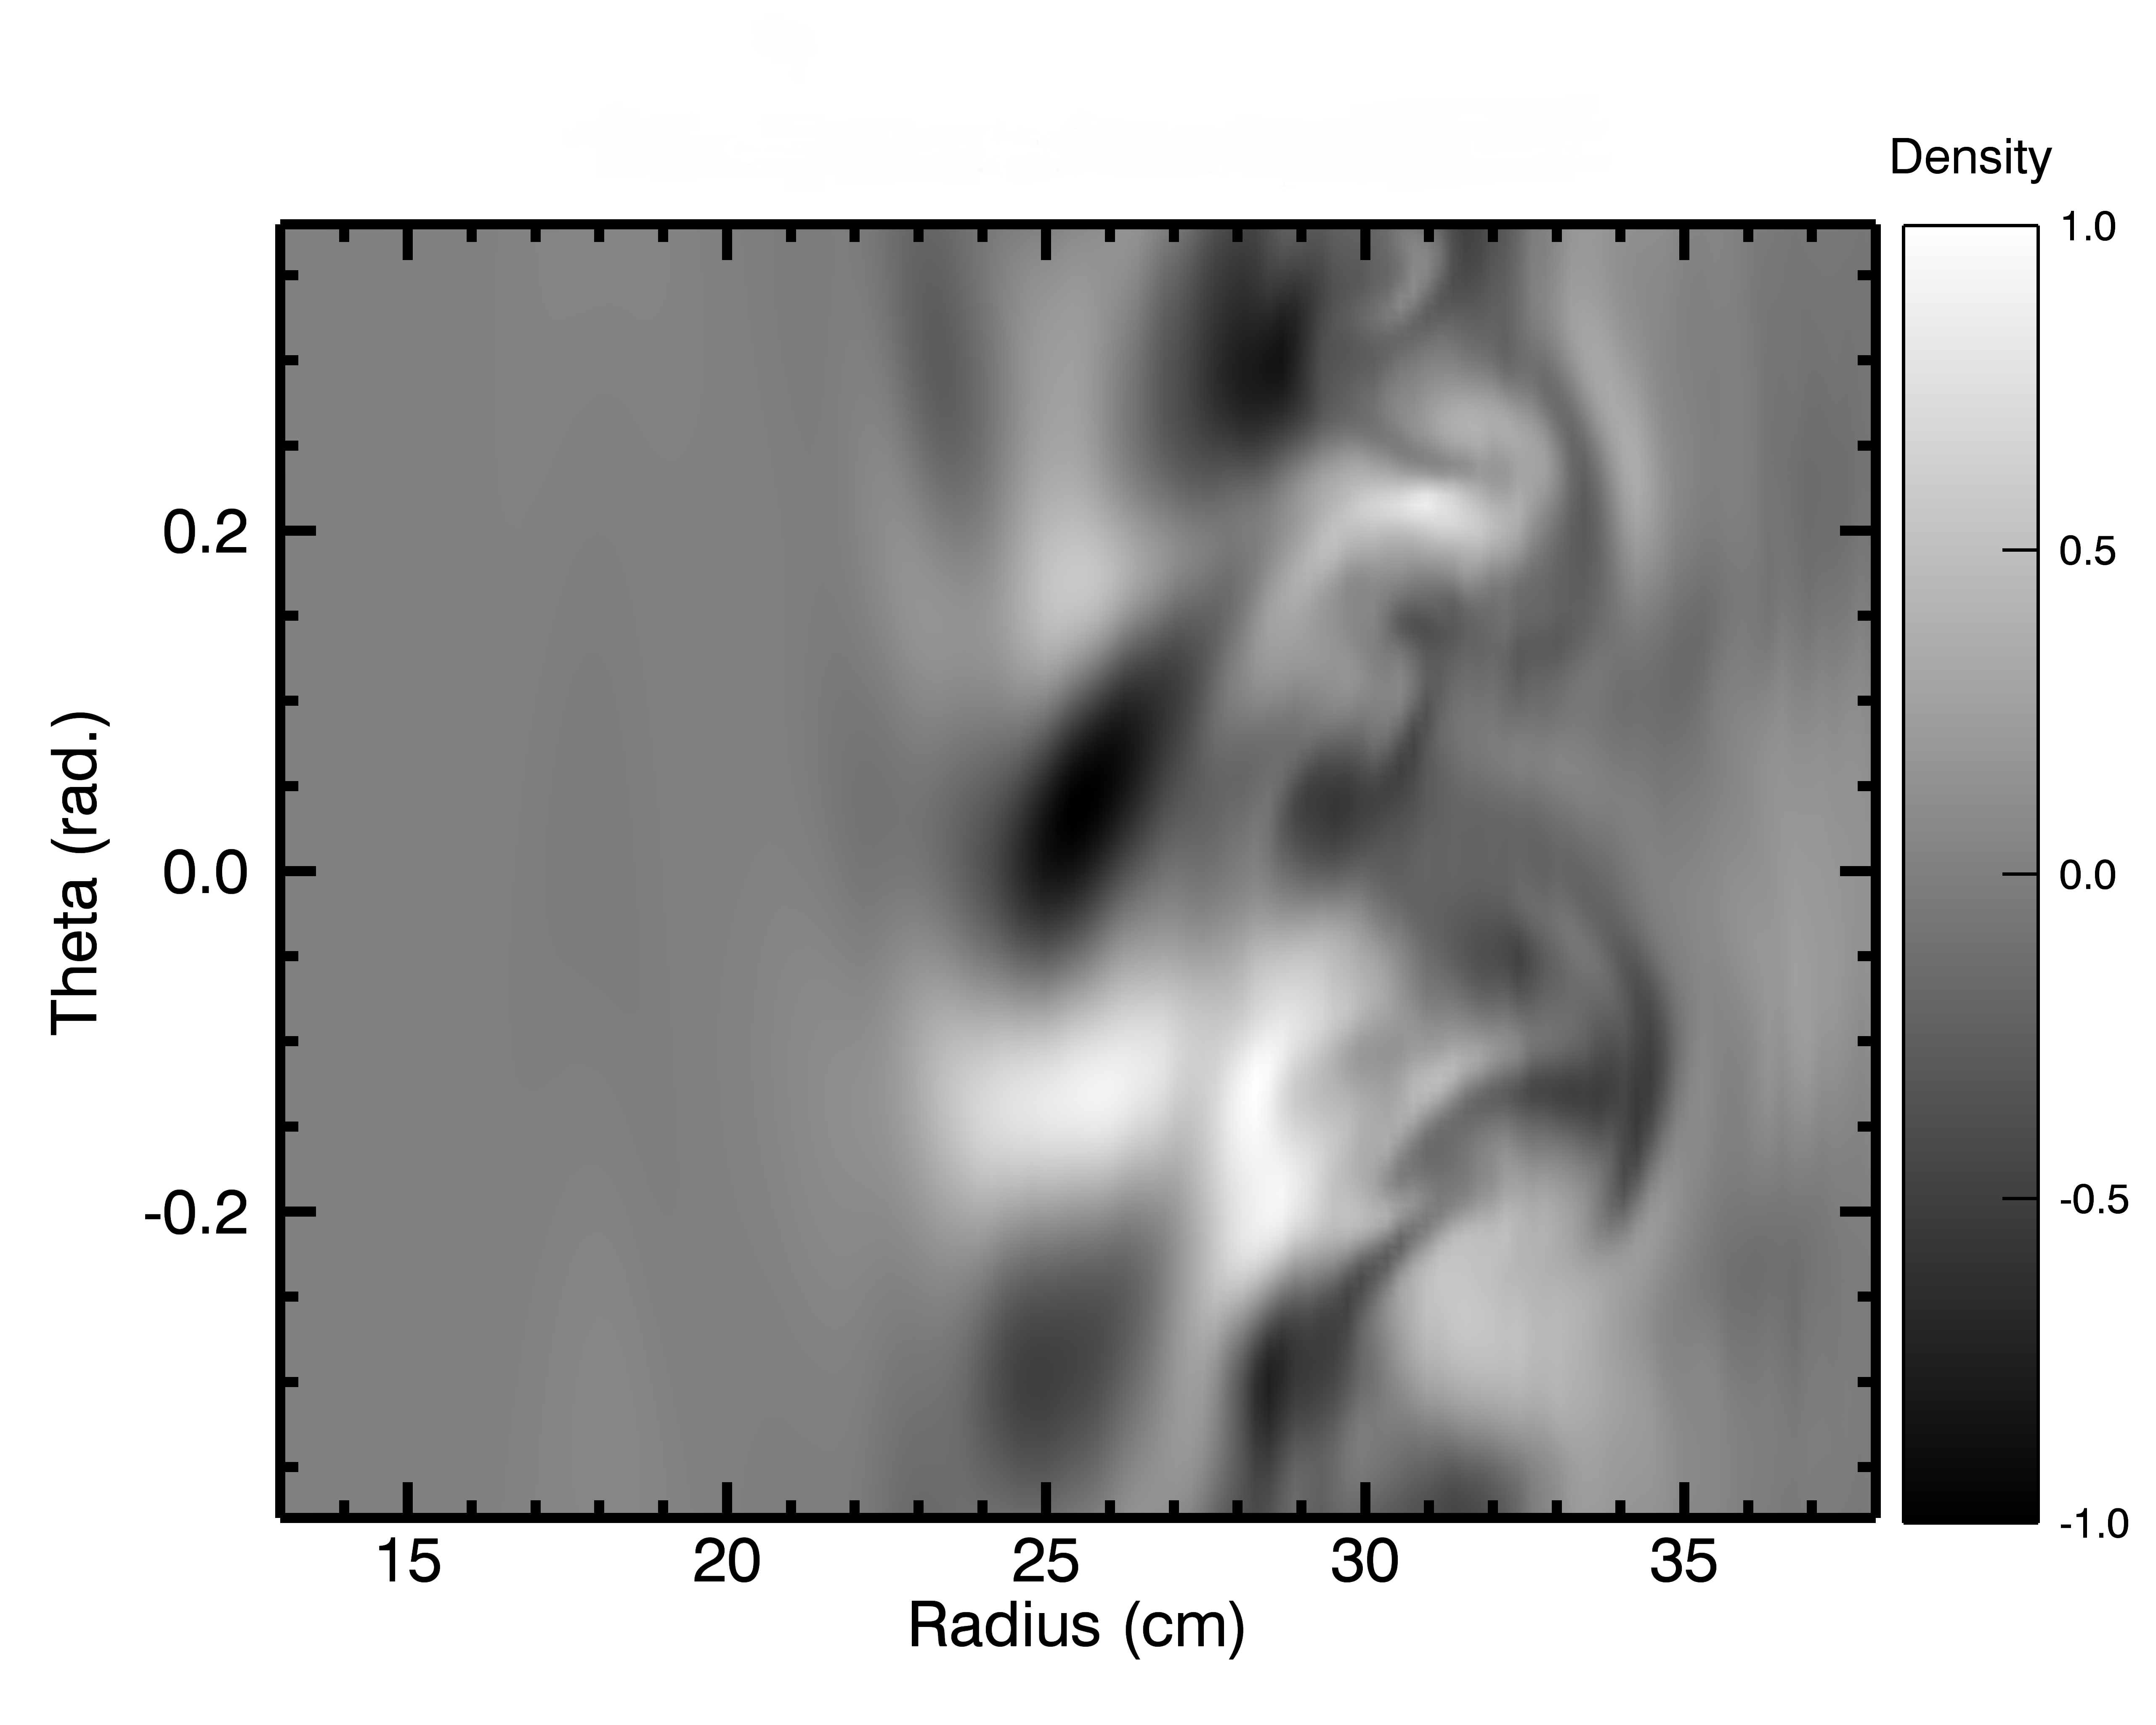
\includegraphics[width=8.5cm]{plot_Bout_contour_for_paper}}
\caption{ A contour of mean subtracted normalized density data of the LAPD, generated by the BOUT++ simulation code.}
\label{fig:plot_Bout_contour_for_paper}
\end{figure}

Simulation data was generated from the BOUndary Turbulence (BOUT++) simulation code. BOUT$++$ is a 3D collisional fluid simulation code modified to treat the cylindrical geometry of the LAPD \citep{popovich10, friedman12, friedman13}. The simulation gives density, temperature, and potential at each point in space and time. To approximate the line integration of light that the camera records, the BOUT data was averaged over the axial direction of the cylinder. This gives a 2D cut of the cylinder of plasma to be analyzed in a similar manner as the camera data would be. An example of the density data has been plotted in Figure~\ref{fig:plot_Bout_contour_for_paper}. In this instance, the program was setup to simulate a large driven $E \times B$ flow in the LAPD. The "frame rate" of the simulation was chosen to be 140 kHz about the same as the fast framing camera. Using the fact that the luminosity is highly correlated to the density, the density field generated by the BOUT simulation is used as the camera field of view. The wavelet method was then used on this density field to calculate a velocity field. Next, the potential field generated from BOUT was also used to calculate the azimuthal flow by calculating the electric field. These two velocity calculations are compared in Figure~\ref{fig:plot_bout_wavelet_vel}, by taking a time and space averaged radial cut of the azimuthal velocity. The wavelet calculations are in fairly good agreement with the traditional calculation from the plasma potential. In Figure~\ref{fig:plot_Bout_contour_for_paper} it can be seen that the density fluctuation structures are non-uniform in size across the field of view. Comparing the density contour to the velocity plot, it can be seen in the regions of large structure size that the velocities do not quite match between the two methods. The structure that dominates this region has a smaller $k$ than is resolvable by the wavelet method. Where the smallest $k$ is given by $1/(n*dx)$, where $dx$ is the distance between spatial points and $n$ is the number of points. In order to resolve this region, one would need a larger field of view that encompasses this structure size. This is a key point to keep in mind when using this wavelet method. One needs to choose an appropriate field of view when dealing with a specific k-spectrum. This demonstrates one of the limitations to the wavelet based method for calculating velocity fields.

\begin{figure}
\centerline{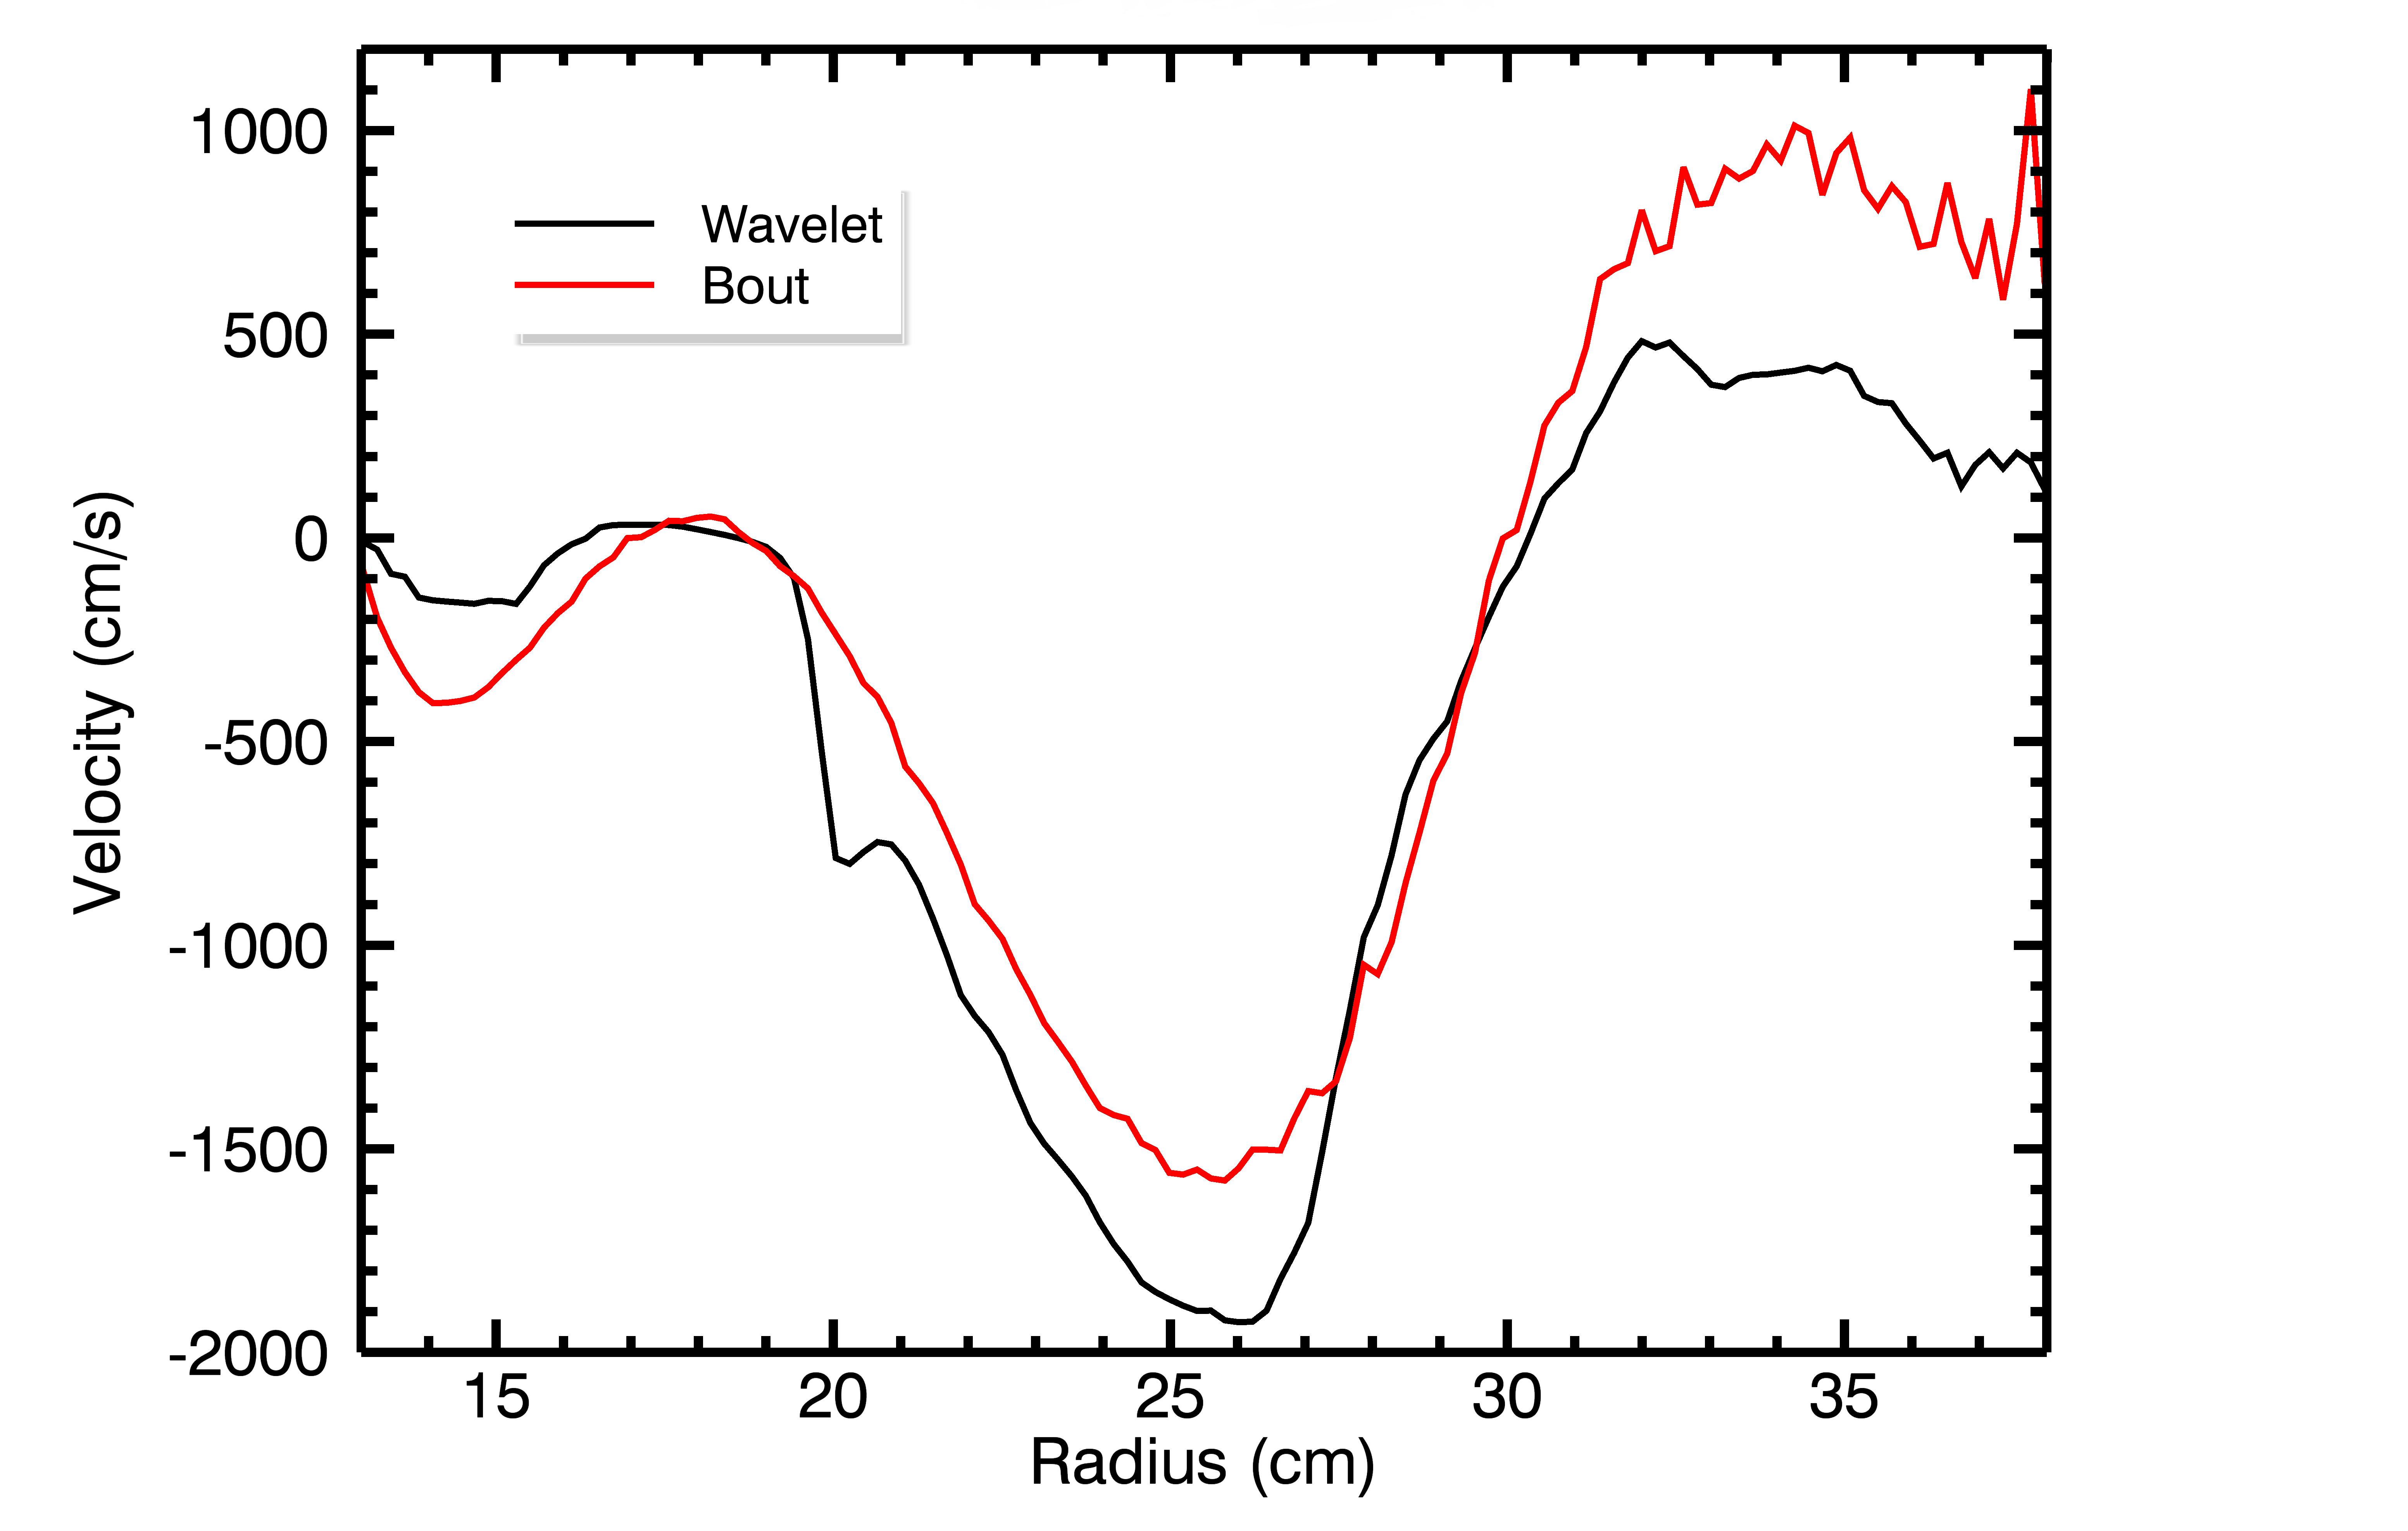
\includegraphics[width=8.5cm]{plot_bout_wavelet_vel}}
\caption{Mean velocity profile calculated from the wavelet method applied to BOUT density data, and velocity profile calculated from BOUT potential data.}
\label{fig:plot_bout_wavelet_vel}
\end{figure}


\subsection{Application to Fast Camera Data}

\begin{figure}
\centerline{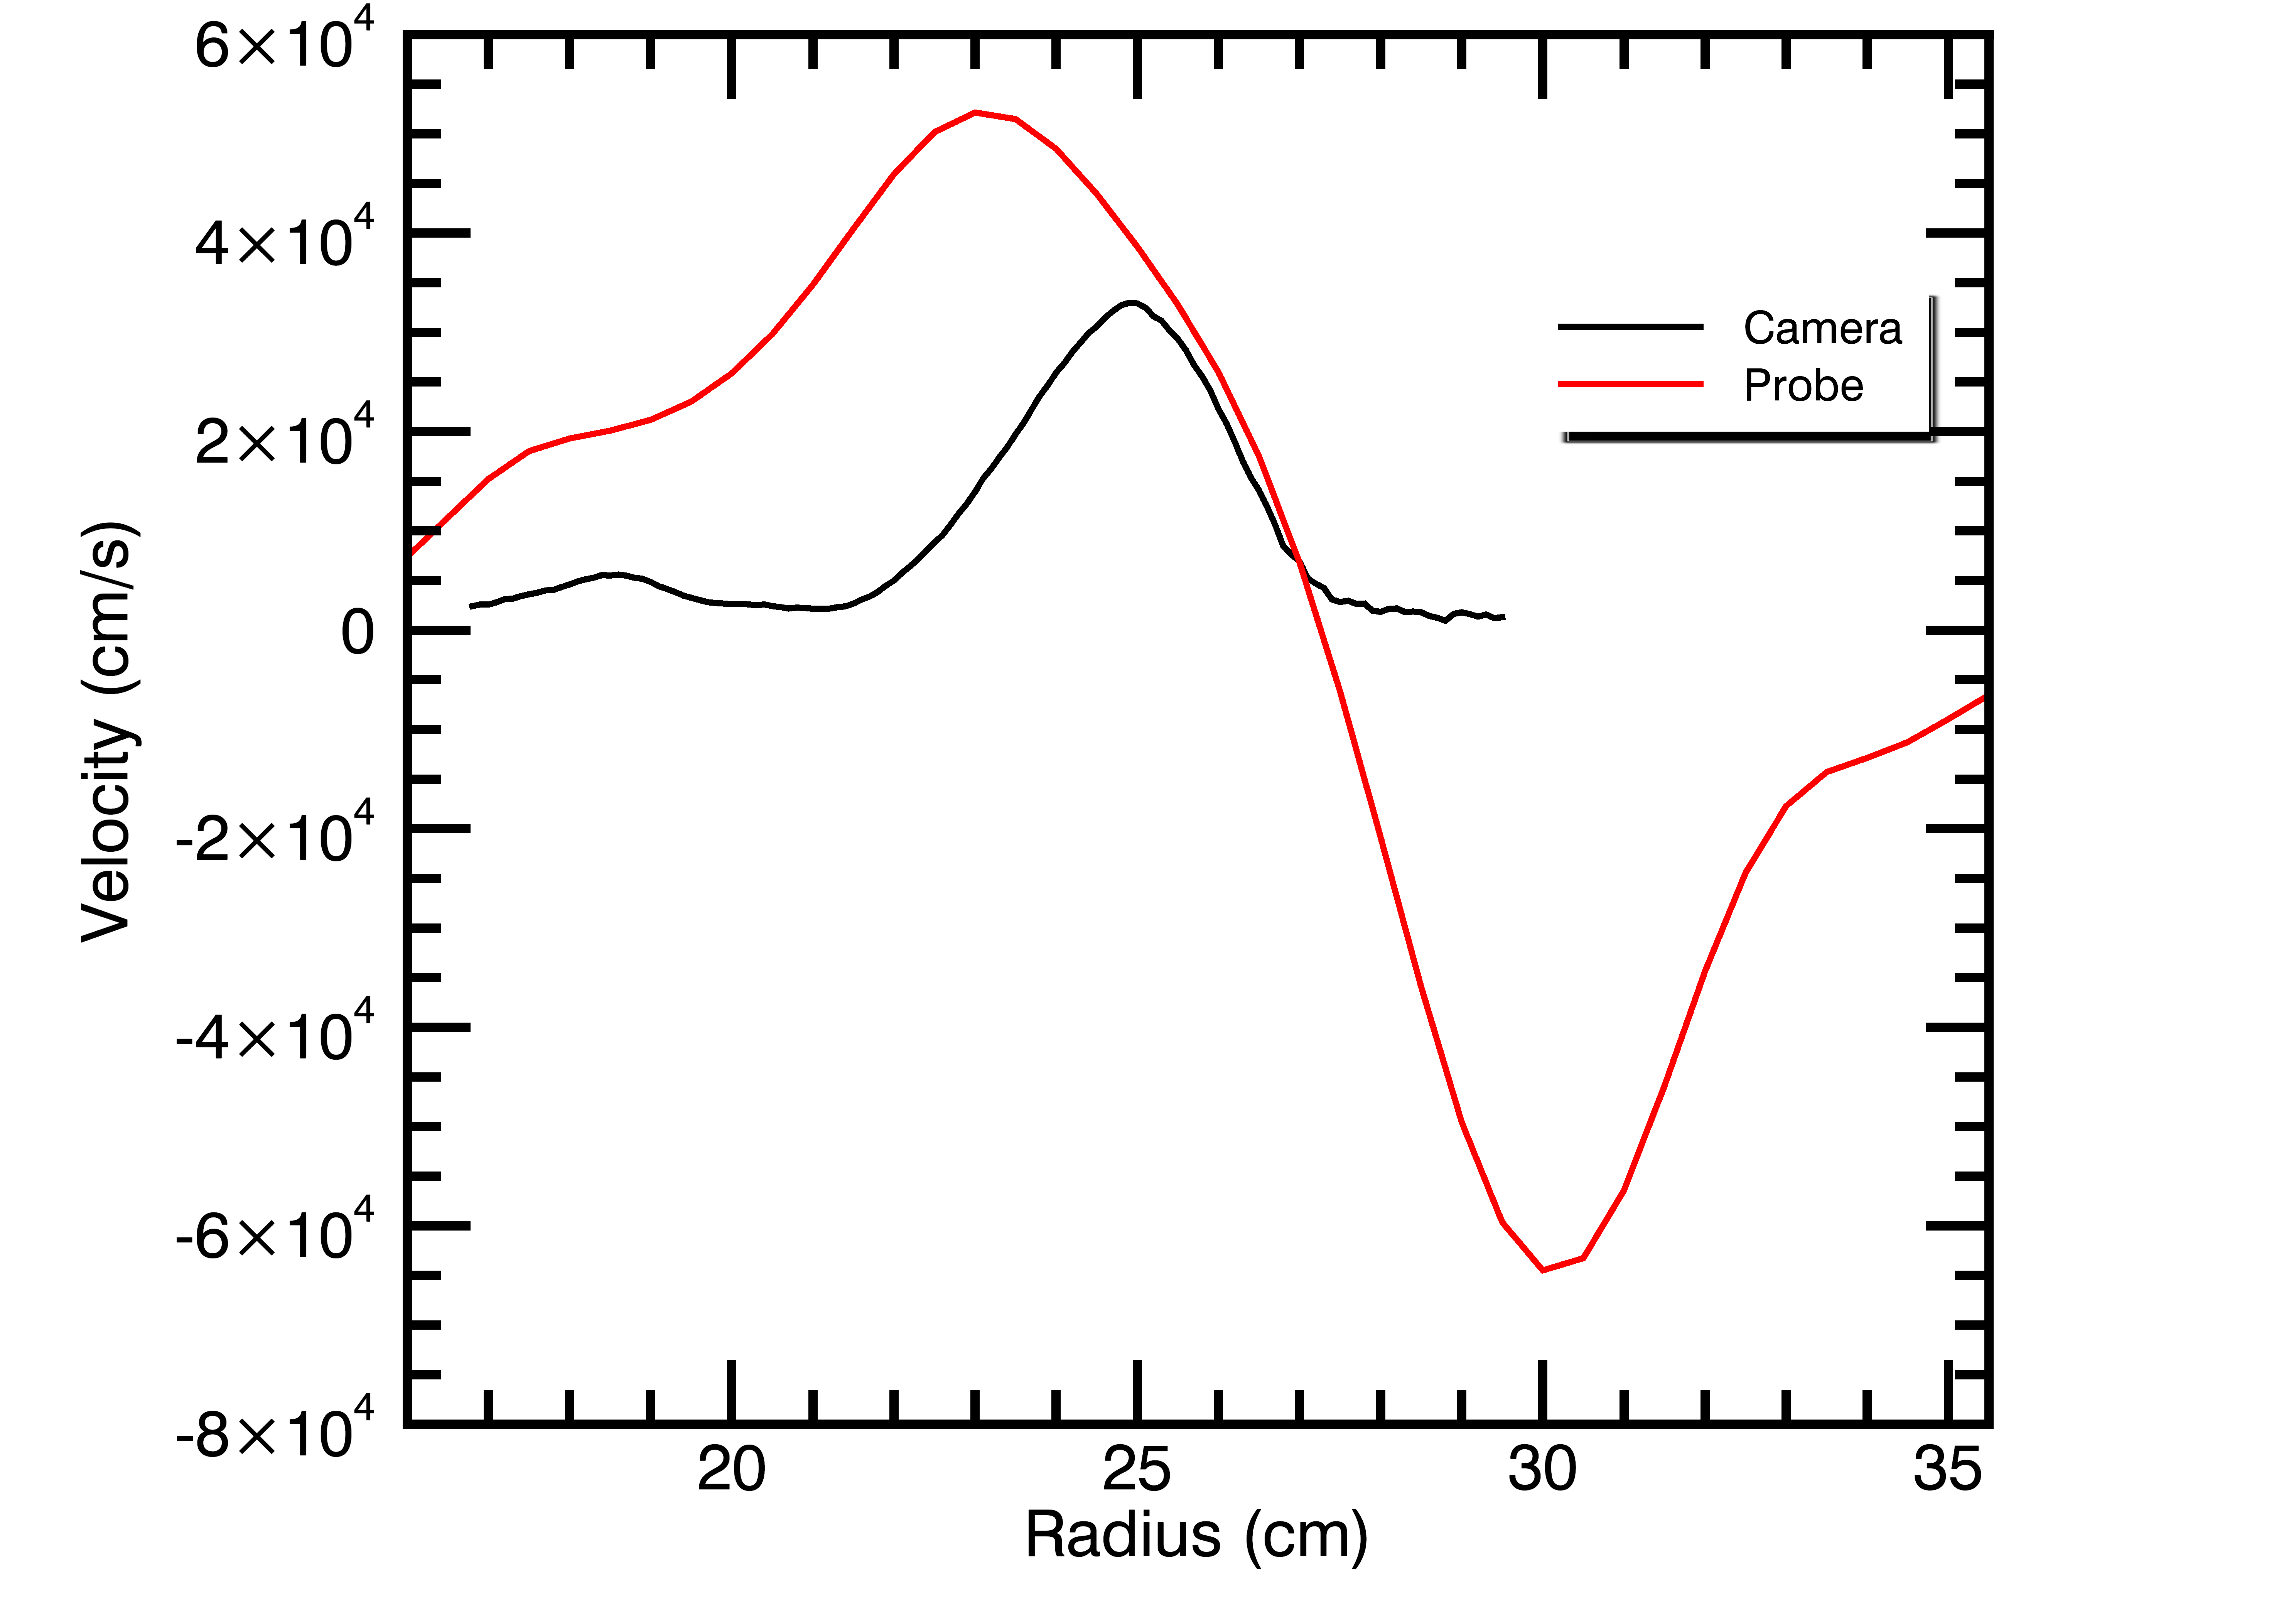
\includegraphics[width=8.5cm]{plot_Velocity_cam_probe_bias_120V}}
\caption{ Mean velocity profiles measured by a swept Langmuir probe and fast framing camera.  A bias of 120V was applied to the limiters causing a strong flow in the EDD radailly inside of the limiter.}
\label{fig:plot_Velocity_cam_probe_bias_120V}
\end{figure}



The wavelet based method is next applied to camera data taken on the LAPD. Again the periscope setup was used and was centered at a radius of 23cm. The time averaged azimuthal velocity profiles calculated from the camera data is plotted along with velocity profile calculated from the swept Langmuir probe in Figure~\ref{fig:plot_Velocity_cam_probe_bias_120V}. In this case the bias of 120V on the limiter was greater than the voltage of the anode creating a flow in the EDD direction.  It can be seen that the velocity profiles do not match very well over much of the profile.  But most of these differences can be explained by different effects seen by the camera.  First looking at the radii greater than 27cm for the camera, the velocity calculation flattens out and becomes noisy.  These effects are caused by the low luminosity seen in this region, which is in turn caused by the drop in temperature and density behind the limiter plates.  For the region inside the limiter edge the plasma is uniformly illuminated and thus there is very little structure for the wavelet method to detect.  It is only in the region most nearest to the limiters edge, both inside and outside, that the method works reasonably well due to the presents of fluctuations in the luminosity.   Velocity profiles have been looked at for many different biases in both the IDD and EDD directions and similar results to Figure~\ref{fig:plot_Velocity_cam_probe_bias_120V} are seen. In Figure~\ref{fig:plot_Velocity_at_25cm_camAt23cm_biasScan} the  velocity at 25cm is plotted at each bias for both the Langmuir probe and the fast camera.  Both diagnostics have the same trend from negative velocities (IDD) to the reversal of flow in the positive direction (EDD). Both the application to BOUT++ and camera data show that this method works in calculating mean velocities, but with some limits.  As for fluctuating velocities, we are currently exploring different methods for comparison, one of which is radial particle flux. Particle flux in the LAPD has traditionally been measured using Ion saturation current as a measurement of the density fluctuations, and velocities were measured by taking the difference in potential between two spatially separated floating potential probe tips. In the case of the camera, we have used luminosity for density and have derived the velocity using this wavelet method.  Measurements of Reynolds stress are also being compared. 

\begin{figure}
\centerline{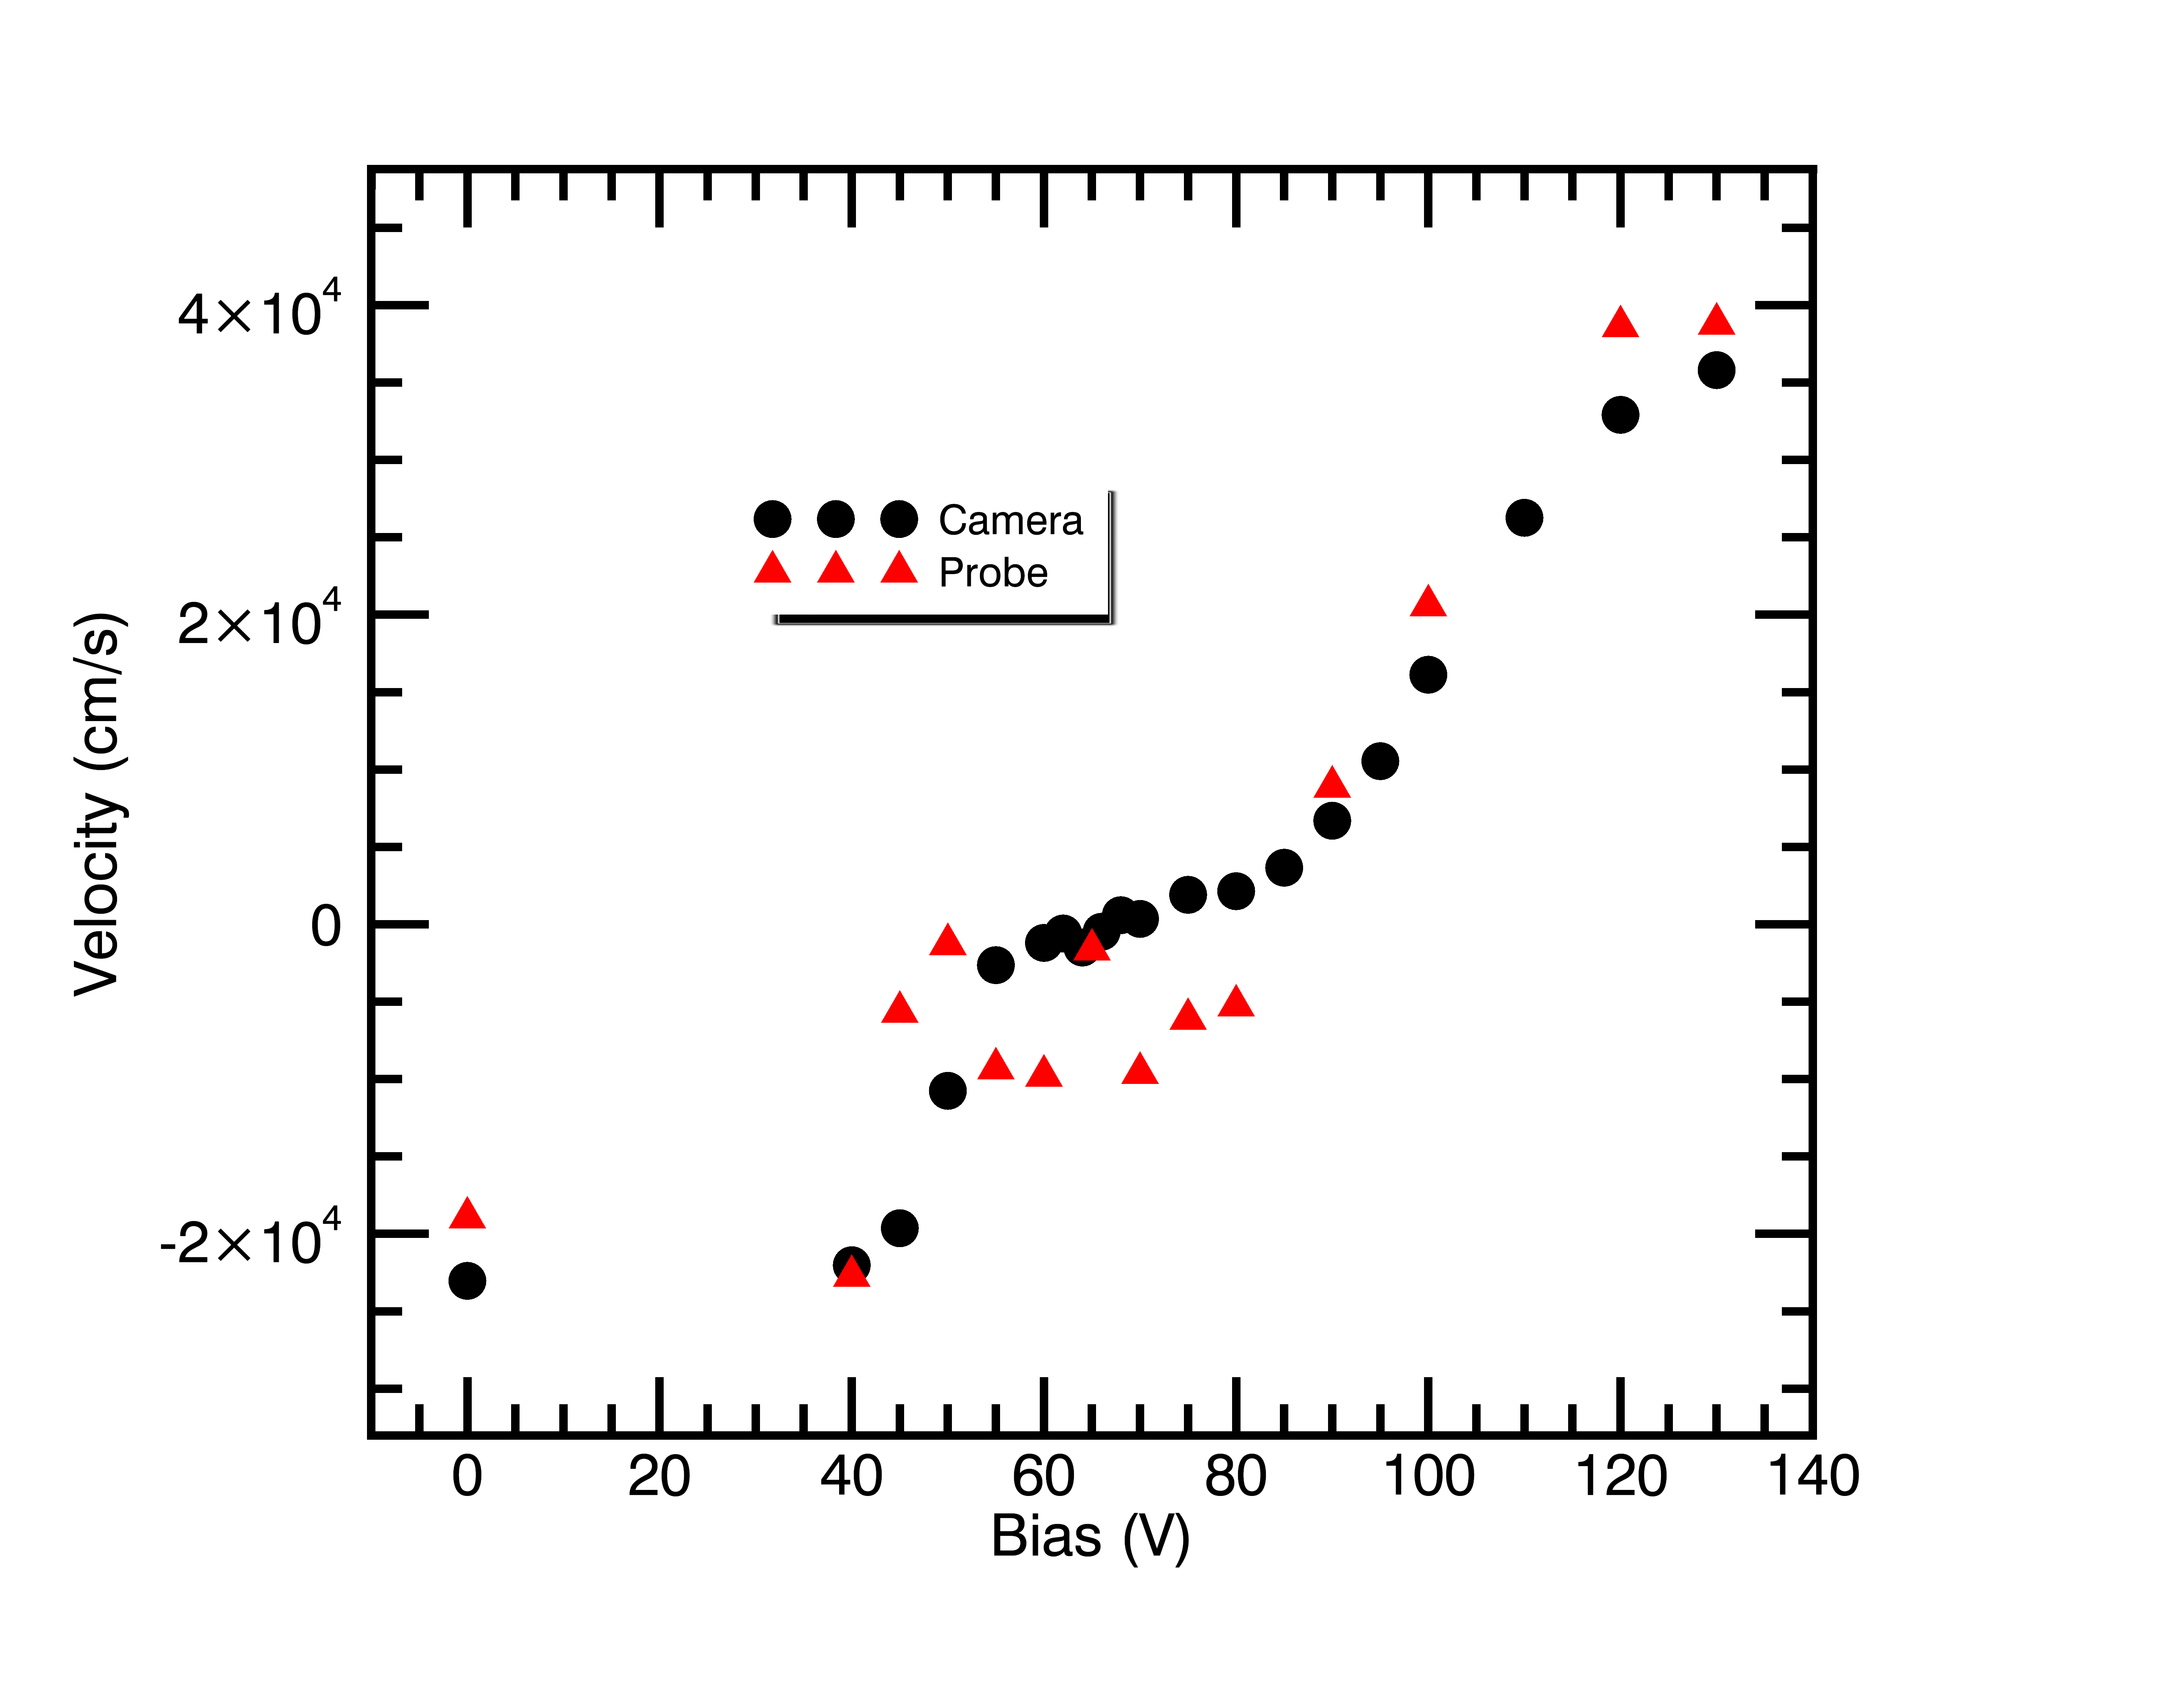
\includegraphics[width=8.5cm]{plot_Velocity_at_25cm_camAt23cm_biasScan}}
\caption{ Velocities calculated by the camera and probe at a radial distance of 25cm for different biases.  The flow can be seen going from the negative direction (IDD) and reversing (EDD) as the bias goes up.  A null flow state is also seen at about 65V.}
\label{fig:plot_Velocity_at_25cm_camAt23cm_biasScan}
\end{figure}


\section{Conclusions}

We have shown that the luminosity measured by the camera has a high correlation with the ion saturation current measured by a triple probe in the LAPD plasma at multiple locations and applied biases. Thus, establishing a physical link between the luminosity and the plasma. While the time averaged camera intensity and density do not agree over all radii, the intensity fluctuations are still assumed to be approximately density fluctuations.  The drop temperature of the plasma behind the limiter edge affects the luminosity levels, so caution must be taken in this region.  It should also be noted that the images taken inside the limiter also have small fluctuations in luminosity.  In the future multiple exposures in multiple regions will be taken to make the useful radial region as large as possible for the camera diagnostic.  

A wavelet based technique used to extract velocity fields from density and luminosity data.  This technique was tested and validated on BOUT++ density simulation data with great success.  This same technique was used on camera data from the LAPD with limited but encouraging results.  The method was limited to a small region of comparison to a Langmuir probe due to the cameras ability to pick up luminosity fluctuations aver a small radial region.  In general one must take precautions when using this wavelet method to choose a correct parameter regime and camera exposure that will yield good results. 

 
The authors would like to thank Marvin Drandell and Zoltan Lucky for their help in designing and building the periscope system used in this experiment and their valuble technical support around the lab.  This work was supported by (fill in) and performed at the Basic Plasma Science Facility (BaPSF) at UCLA.  The BaPSF is funded by the Department of Energy and the NSF. 





\bibliographystyle{jpp}
% Note the spaces between the initials


\bibliography{jpp-fast_camera}

\end{document}
